\documentclass[%
aip,
%jmp,%
%bmf,%
sd,%
%rsi,%
amsmath,amssymb,
preprint,%
%reprint,%
author-year,%
%author-numerical,%
]{revtex4-1}
\usepackage{graphicx}% Include figure files
\graphicspath{ {figures/} }
\usepackage{dcolumn}% Align table columns on decimal point
\usepackage{bm}% bold math
\usepackage[mathlines]{lineno}

%\linenumbers\relax % Commence numbering lines

%\draft % marks overfull lines with a black rule on the right
\usepackage{color}
\usepackage{bm}
\usepackage{booktabs}
\usepackage{makecell}
\usepackage{multirow}
\usepackage{float}
\usepackage{color}
\usepackage{tikz}
\usetikzlibrary{shapes}
\usepackage{amsmath}
\usepackage{lipsum}
\usepackage{gensymb}
\begin{document}
\newcommand{\MarkerCircleRed}{\raisebox{0.5pt}{\tikz{\node[draw,scale=0.4,circle,fill=red!100!red](){};}}}
\newcommand{\MarkerSquareRed}{\raisebox{0.5pt}{\tikz{\node[draw,scale=0.4,regular polygon, regular polygon sides=4,fill=black!20!red](){};}}}
\newcommand{\MarkerDiamondBlack}{\raisebox{0pt}{\tikz{\node[draw,scale=0.4,diamond,fill=black!100!](){};}}}


\title{Liquid Chain Genesis by Collision of Two Laminar Jets}
\author{Vatsal Sanjay}
\email{vatsalsanjay@gmail.com}
\author{Arup Kumar Das}
\email{arupdas80@gmail.com}
\affiliation{Department of Mechanical and Industrial Engineering, Indian Institute of Technology, Roorkee}
\date{\today}

\begin{abstract}
Liquid chain genesis is studied through a series of fully resolved numerical simulations. Transient process of collision of liquid jets and subsequent formation of sheet in a plane perpendicular to the impinging jets is illustrated and analyzed to pertain towards a steady state in which a chain like fluidics structure is formed, with subsequent sheets forming the respective links of the chain in mutually orthogonal planes. Two different models using regression and analogy of billiard balls collision, are proposed to predict the shape and size of the first link. On one hand, the former gives information about the dimensions of the link to a better accuracy, the latter force balance model using the billiard balls analogy gives an insight into the Physics of the problem. Further, the flow kinematics is studied with self-similar velocity profile in the sheet and the effects of different physical properties on the average sheet velocity. At last, special attention is given to the second collision that forms a liquid sheet orthogonal to the first one and the mode of collision can be generalized for the entire chain structure.     
\end{abstract}
\keywords{Impinging jets, Liquid sheet, Fluid chain}
\maketitle
\section{Introduction}\label{Sec::Introduction}
\begin{figure}[H]
	\centering
	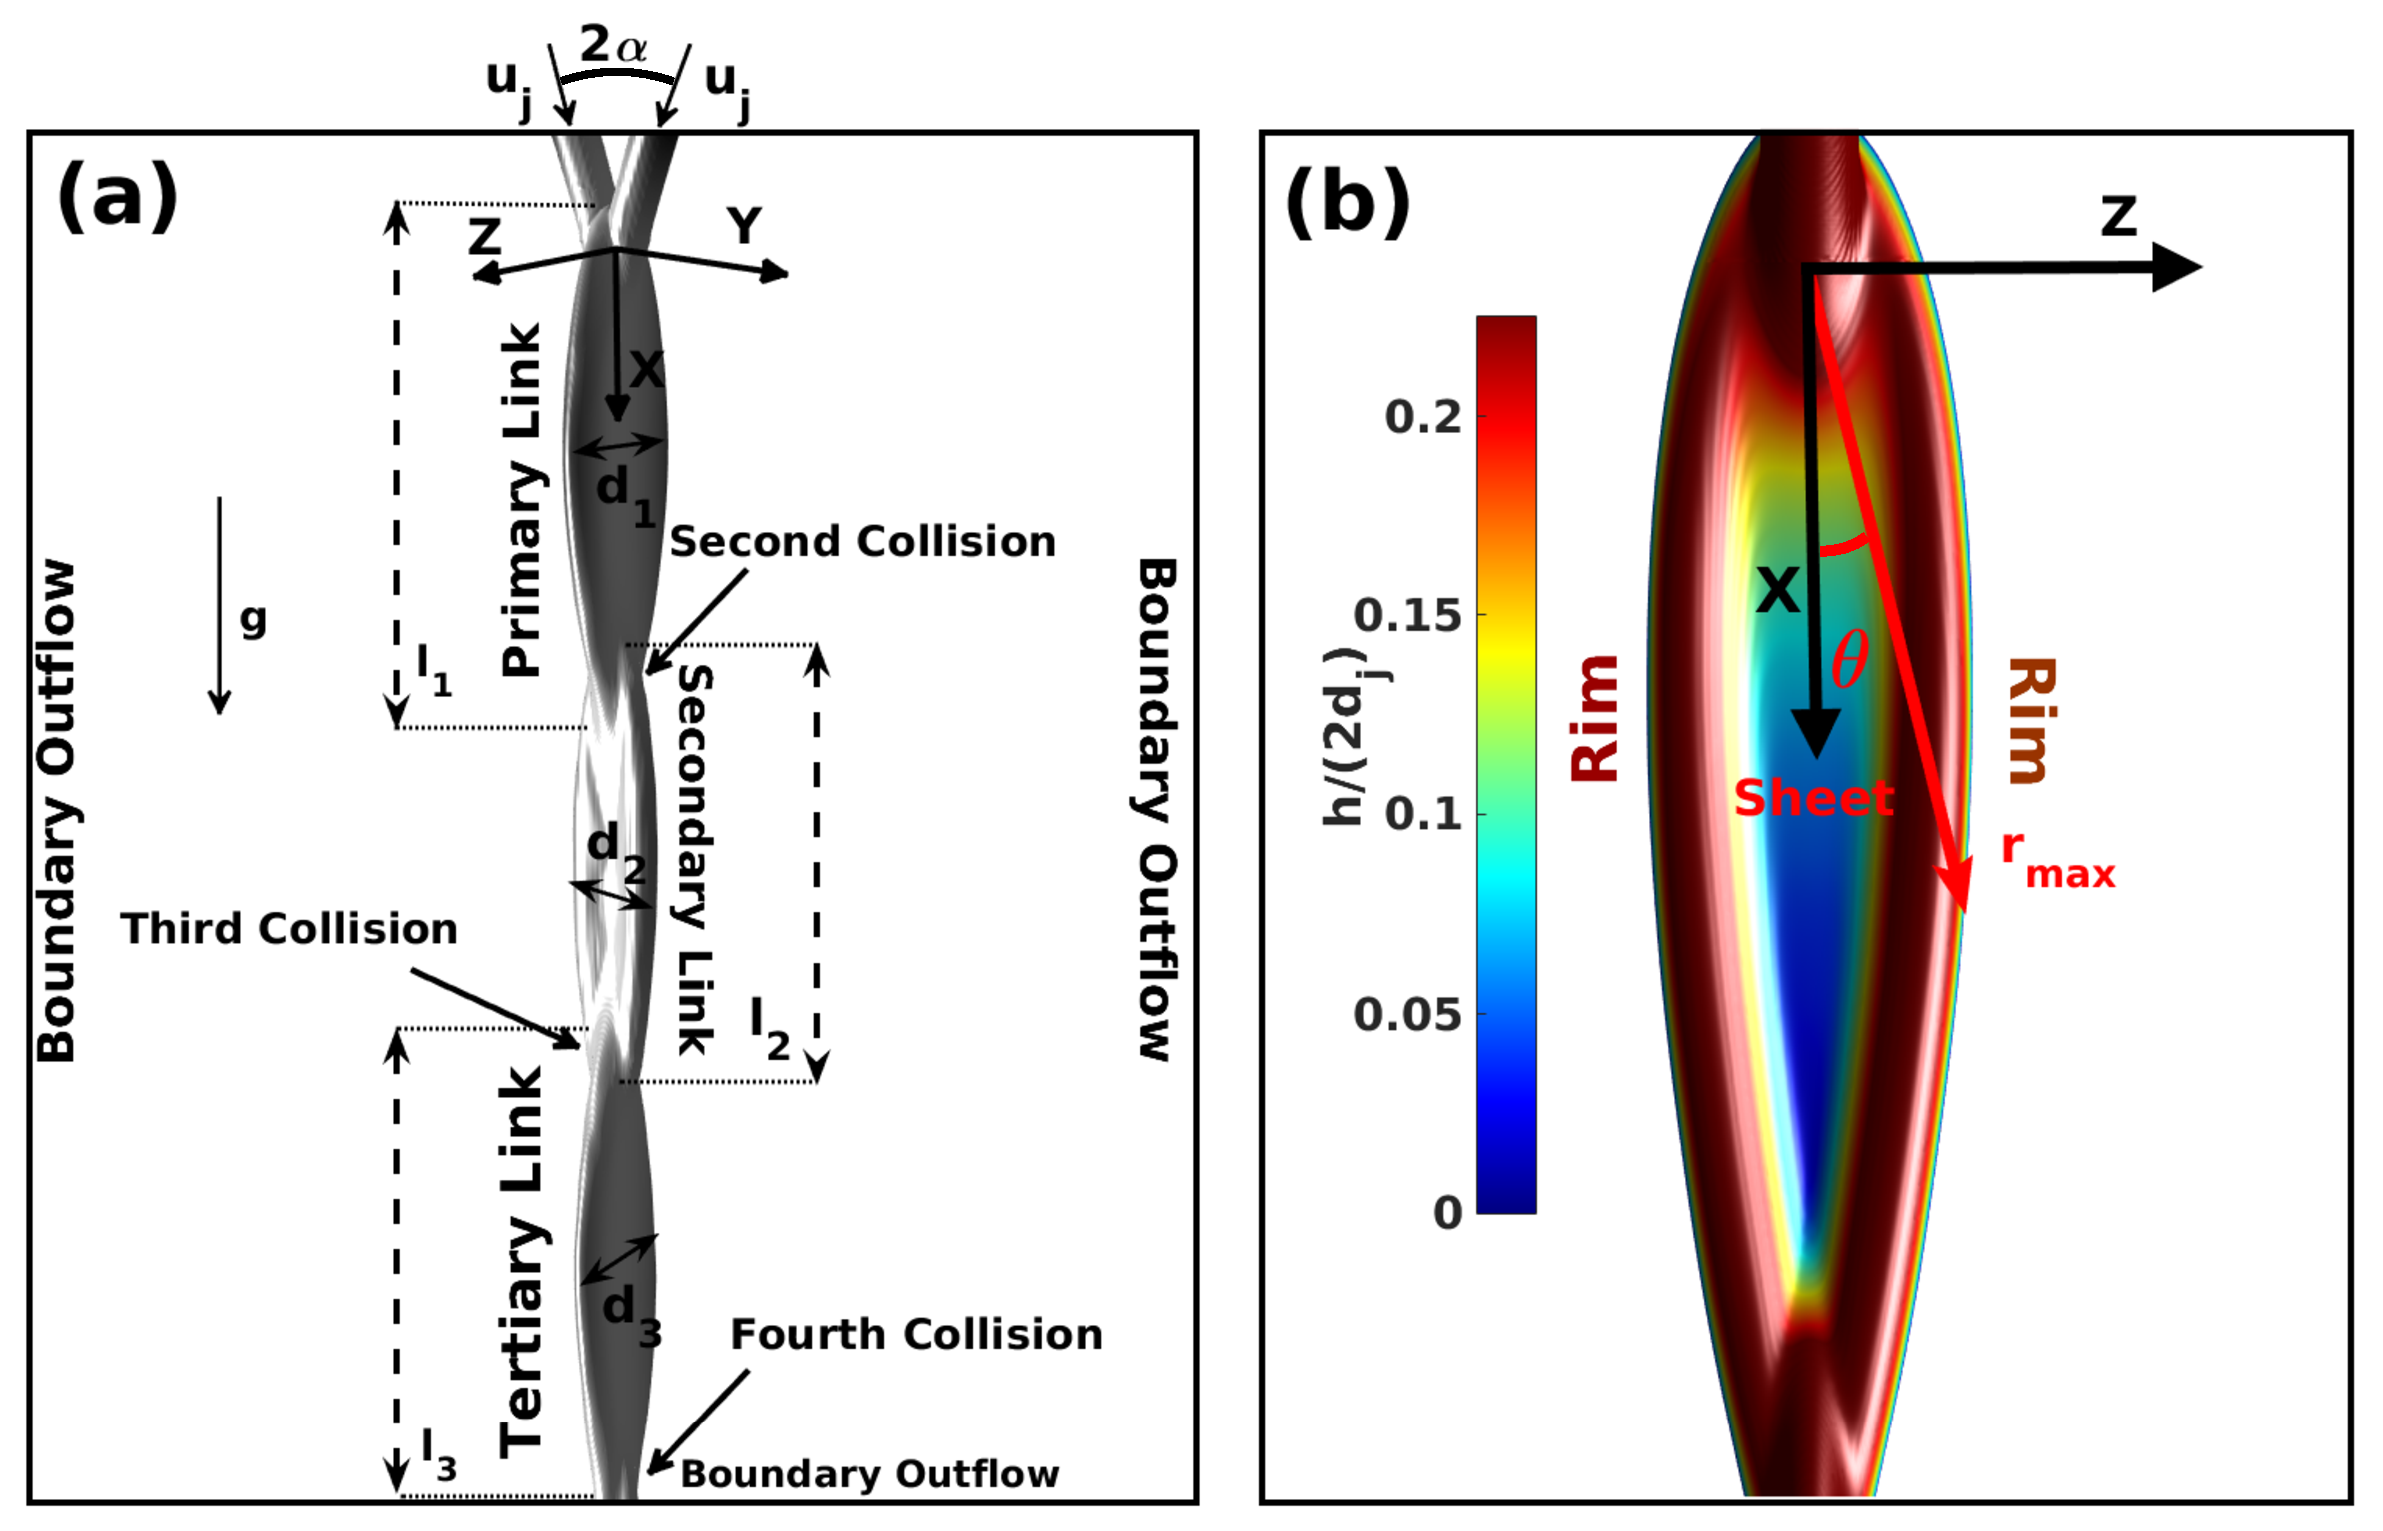
\includegraphics[width=0.6\linewidth]{schematic}
	\caption{Formation of the liquid sheet by collision of laminar jets. A schematic to illustrate different structural features and length scales. The mutually perpendicular sheets mark different links of the fluid chain structure.}
	\label{Figure::schematic}
\end{figure}
Interactions of liquid jets have invoked the curiosity of researchers with their ubiquitous presence \citep{eggers2008physics} ever since the 16$^{th}$ century, eminent in the works of Leonardo Da Vinci as reported by \cite{da1999codex}. One of these interactions is the collision of liquid jets presented by \cite{rayleigh1879capillary} and the references therein. Collision of impinging jets result in formation of a liquid sheet perpendicular to the plane of the jets. \cite{bush2004collision} introduced several regimes to characterize the different flow structures obtained from such collisions, working on the theory of liquid jet impingement given by \cite{taylor1960formation}. At low velocities or small angles of impingement (near to vertical jets), the two jets may coalesce to form a single jet or bounce off due to presence of a thin film of air between them \citep{wadhwa2013noncoalescence}. The recoil of such jets is surface tension dominated. On increasing the flow rates, laminar jets may lead to formation of a stable liquid sheet bounded by a thick rim \citep{yang2014liquid}. Inertia and body forces (gravity) act to expand the liquid sheet formed but the action of surface tension force puts a check on this expansion and the sheet converges, such that the successive collisions of the thick rims downstream of the flow result in formation of mutually orthogonal liquid sheets \citep{bush2004collision}. Figure~\ref{Figure::schematic} illustrates this structure which has been termed as the liquid chain with the complementary orthogonal sheets forming the different links. As the velocity of the jets is increased, Kelvin - Helmholtz type of instability takes control \citep{bremond2006atomization}, resulting in the formation of destabilizing waves \citep{villermaux2002life} which leads to ejection of droplets from the liquid rim featuring Plateau-Rayleigh instability through mechanisms explained by \cite{lhuissier2011destabilization}. Further increase in velocities marks the transition of the regime from fluid fishbones into vigorously flapping sheet leading to atomization \citep{ibrahim1991impinging}. This process has been employed as an efficient method of fuel injection system in liquid propellant rocket engines because of its high mixing efficiencies. Unsurprisingly, most of the works on collision of liquid jets revolve around the regime of atomization \citep{miller1960distribution,ibrahim1991impinging,bremond2006atomization,chen2013high,zheng2015numerical}. Among these regimes, we explore the formation of stable closed liquid sheets and the consequent chain structure (Figure~\ref{Figure::schematic}). \\
A wide range of experimental works can also be found which explores the formation of stable liquid sheets using viscous jets. Emphasis has been given on predicting the shapes of the leaf-like links formed in the chain structure and results of model by \cite{bush2004collision} give a remarkable correspondence with the experimental observations. However, the model requires input from the experiments in order to close the system of differential equations. The results from their work have been used to validate our mathematical model in Section~\ref{section::valid}. The formation of these links in the chain structure is extremely sensitive to the initial velocity profile of the liquid jet at the entry of domain as argued by \cite{choo2002velocity,choo2007effect,inamura2014effect}. Experiments show that the jet velocity near the inlet plane follows a parabolic profile \citep{choo2002velocity}. Incorporation of this velocity profiles for laminar jets can refine the results obtained  with the numerical simulations \citep{chen2013high}. Therefore, a fully developed parabolic velocity profile has been adapted for the laminar liquid jet at inlet as discussed in the Section~\ref{Section::Numerical}. Further, using Particle Image Velocimetry (PIV) technique, radial streamlines are observed near the point of impingement and the fluid parcels travel towards the periphery resulting in the formation of the thick rim because of fluid accumulation \citep{choo2002velocity,bush2004collision}. The rim is stable as long as the curvature force developed by surface tension provides the necessary centripetal acceleration as the fluid packets in the rim accelerate owing to loss in gravitational potential \citep{bremond2006atomization}. On balancing the two, \cite{taylor1960formation} developed an expression for the sheet radius, given by $r_{max} = \rho u_0 Q(\theta)/(2\sigma)$ (where, $u_0$ denotes the average sheet velocity, $Q(\theta)$ implies the liquid flux distribution within the sheet and $\rho$ and $\sigma$ are the fluid density and surface tension coefficient with air respectively) and has been found to describe the experimental results of \cite{bush2004collision}.  However, in most of the numerical work done so far, the velocity of the liquid sheet has been assumed to be constant and effect of forces because of viscosity of the fluid and drag offered by surrounding air medium are neglected \citep{taylor1960formation,hureau1998impinging,bush2004collision}.\\ It is necessary to investigate the phenomenon with a fully resolved closed form solution of the Navier-Stokes equations in a three dimensional framework. \cite{chen2013high} used an improved Volume of Fluid technique with Adaptive Mesh Refinement (AMR) coupled with the Finite Volume Method to delve into the different regimes of flow structures formed on collision of liquid jets, from the stable chain structure to violent flapping liquid sheet atomization. We use the same mathematical model with efforts to concentrate on the fluid chain regime with attempts to understand the flow inside the sheet and characteristics of the first link. Special attention is also provided to the mechanism of formation of the secondary links of chain structure, which can be extended to the tertiary links as well. \cite{chen2013high} validated the numerical model with the results from the theoretical works of \cite{bremond2006atomization}, and we have carried out a similar validation with the experimental results of \cite{bush2004collision}. Apart from \cite{chen2013high}, there have been only a few other works for the numerical simulation of the process, owing to the complexity that arises due to multiple length scales (from the jet diameters $\left(d_j\right)$ to liquid sheet thickness $\left(\sim 10^{-2}d_j\right)$). \cite{inoue2008study,inoue2009liquid} attempted to simulate the atomization regime of liquid jets collision with less than 50 grid points across the diameter of the jets, leading to inability in tracking of the small scale droplets and sheet thickness way downstream of the point of collision. Other works include the simulations by \cite{arienti2012coupled} which is also in the atomization regime, whereby the combined level-set and volume of fluid technique \citep{sussman2007sharp} was used coupled with Lagrangian Point Particle (LPP) tracking for the small scaled droplets. Recently, \cite{da2016surface} developed an innovative technique for simulations using surface only fluids, whereby only surface velocity fields are solved using the Boundary Element Method (BEM) on a three dimensional framework, but suffers from the same inviscid assumption taken in earlier theoretical works. Moreover, an extensive work on the chain structures with proper characterization is required. In the present work, we attempt at presenting an overall behavior of the fluid chain structure while focusing on the Physics of flow for the first link by analyzing the dimensional characteristics and velocity field. Special attention is given to the secondary collision, leading to the formation of the subsequent mutually orthogonal links. In the next section, the numerical framework employed in this work is explained followed by the mesh sensitivity analysis and validation in Section~\ref{section::valid}. 

\section{Numerical Formulation}\label{Section::Numerical}
%% Introduction to the problem
Collision of liquid jets has been studied using three-dimensional two-phase flow simulations using the finite volume framework for discretization and Volume Of Fluid (VOF) approach for interface tracking. Open source time-dependent, multi-fluid Navier-Stokes solver, Gerris is used for the current study \citep{Popinet2003}. Gerris has been successful used frequently by researchers, such as \cite{chen2013high,kumar2016physical,kumar2017bending}, to delve into similar problems in interfacial flows involving liquid sheets, jets and thin features like ligaments and films to capture intricate flow details and investigate the process. It invokes an adaptive mesh projection method for solution of incompressible continuity and momentum equations. The spatial discretization of the domain is undertaken using an octree based structured hierarchal grid system, which can be locally refined. Equation~\ref{Equation::mass} contains the mass conservation equation for the incompressible flow, which simply states that the velocity field ($V_i = V_1\hat{i} + V_2\hat{j} + V_3\hat{k}$) must be divergence free.   
\begin{equation} \label{Equation::mass}
\frac{\partial V_i}{\partial x_i} = 0
\end{equation}
The momentum equation for the incompressible Newtonian fluids that is solved for all three spatial coordinates can be summarized as given in equation~\ref{Equation::NS}. In the equation, the forces applied on the control volume chosen consist of the pressure in form of its gradient field ($\frac{\partial p}{\partial x_i}$), the volume specific body force due to gravitation ($\rho g_i$), the surface forces due to shear stress ($2\mu D_{ik}$, where $\mu)$ represents the coefficient of dynamic viscosity and $D_{ik}$ is the deformation tensor) and the interface specific surface tension force ($\sigma \kappa$, where $\sigma$ is the surface tension coefficient and $\kappa$ denotes the curvature of interface). 
\begin{equation} \label{Equation::NS}
\rho\left( \frac{\partial V_i}{\partial t} + V_k\frac{\partial V_i}{\partial x_k} \right) = -\frac{\partial p}{\partial x_i} + \frac{\partial (2\mu D_{ik})}{\partial x_k} + \sigma \kappa \delta_sm_i + \rho g_i
\end{equation}
Moreover, the surface tension term is multiplied with the Dirac distribution function ($\delta_s$) to ensure that the force by surface tension is concentrated at the interface having the normal vector $m_i$. Further, the deformation tensor $D_{ik}$ is defined using the symmetric part of the velocity field gradient as given in Equation~\ref{Equation::deformation}.
\begin{equation} \label{Equation::deformation}
D_{ik} = \frac{1}{2}\left(\frac{\partial V_i}{\partial x_k} + \frac{\partial V_k}{\partial x_i}\right)
\end{equation}
The Equation~\ref{Equation::NS} (Navier Stokes) implicitly implies the conservation of the mechanical energy. Moreover, the temperature variations are too small to affect the phenomenon being investigated and therefore, no thermal energy equation is employed. The interface tracking is undertaken using the Volume Of Fluid (VOF) approach. For this, a volume fraction (tracer) is defined as $\Psi(x_i,t)$, at the spatial and temporal instance of $x_i$ and $t$ respectively. Therefore, the density and viscosity for the study can be defined as given by Equation~\ref{Equation::general}. The Volume of Fluid approach implemented is a two-step process of interface reconstruction (based on the values of $\Psi$ and piecewise linear interface construction scheme, PLIC) along with geometric flux computation and interface advection. Equation~\ref{Equation::vof} represents the advection equation for the volume fraction field.
\begin{equation} \label{Equation::general}
A (\Psi) = \Psi A_1 + (1-\Psi)A_2 \: \: \:  \forall  \: A \in \{\rho, \mu\}
\end{equation}
\begin{equation} \label{Equation::vof}
\frac{\partial \Psi}{\partial t} + \frac{\partial(\Psi V_i)}{\partial x_i} = 0
\end{equation}
%% Time marching scheme
Second order accurate time discretization of momentum and continuity equations are carried out with time splitting algorithm as proposed by \cite{Chorin1968}, whereby an unconditionally stable corrector predictor time marching approach is adopted. A multi-grid solver is used for solution of the resulting pressure-Laplace equation. The advection term of the momentum equation $\left(V_k\frac{\partial V_i}{dx_k}\right)$ is estimated using the Bell-Colella-Glaz second-order unsplit upwind scheme \citep{bell1989second}, which requires the restriction to be set up on the time step between subsequent time steps based on the Courant-Friedrichs-Lewy (CFL) stability criteria as the estimation is stable only for CFL $<$ 1 \citep{popinet2009}. The details of the octree-based multi-level solver employed for the solution of the system of the equations can be found in the works of \cite{Popinet2003,popinet2009}. \\ 
%% Specific to this problem
Figure~\ref{Figure::schematic} illustrates the computational domain with dimensions 30$d_j$ x 10$d_j$ x 10$d_j$. The lateral surfaces are kept at a distance of $5d_j$ to avoid any biasing from the boundaries. These surfaces along with the bottom one are kept as standard boundary outflow. Two small liquid jets inclined at an angle of $\alpha$ from the vertical are initialized at the start of the simulation. The boundary condition on the top surface of the computational domain is that of liquid jet inlets, for which a parabolic velocity profile $\left(\left[2\left(1 - \left(\frac{2r}{d_j}\right)^2\right) \right]u_j\right)$ is patched, where $r$ is the radial location in the jet from its centerline, $d_j$ is the diameter of the liquid jets and $u_j$ is the average inlet velocity of the jet as illustrated in Figure~\ref{Figure::schematic}. We restrict ourselves in the laminar flow regime as the formation of stable liquid chains or sheet structures with closed rim is prominent in this regime. Following the Equations~\ref{Equation::mass} to~\ref{Equation::vof} and the boundary conditions, one can easily see that different features of these liquid sheets can be represented in terms of the kinematic and dynamic properties, such as jet velocity $\left(u_j\right)$, its diameter $\left(d_j\right)$, angle of impingement $\left(2\alpha\right)$, acceleration due to gravity $\left(g\right)$ and other physical properties, such as density of the fluid $\left(\rho\right)$, its viscosity $\left(\mu\right)$ and the coefficient of surface tension at the fluid-air interface. On dimensional analysis, different independent PI - terms are recognized as given in Equation~\ref{Equation::Pi}. On the left hand side we have different chain and link features, such as the length of individual lengths of the link, its maximum extent in the the plane of the formation of the liquid sheet, the average fluid velocity in the liquid sheet $\left(\:\frac{u_0}{u_j} = \int_{0}^{1}\int_{0}^{1}\int_{0}^{1}\frac{\sqrt{V_iV_i}}{u_j}d\left(\frac{y}{h}\right)d\left(\frac{r}{r_{max}}\:\right)d\left(\frac{\theta}{2\pi}\right) \right)$ and the thickness of the liquid sheet at different spatial locations $\left(\frac{h}{d_j}\right)$. Further, on the right hand side of the equation, different non-dimensional numbers can be recognized based on flow and geometric properties. The first term can be identified as the Froude number $\left(Fr = \frac{u_j}{\sqrt{gd_j}}\right)$, which acts as a measure of the relative strength of the inertia of the liquid jet and the force of gravity. Gravity is taken in the positive x-direction as shown in Figure~\ref{Figure::schematic}. Second term is the Bond number $\left(Bo = \frac{\rho gd_j^2}{\sigma}\right)$, used to account for the strength of the surface tension force as compared with the gravity body force on the chain structure. The viscosity comes into consideration with the term given by $\left(\frac{\mu}{\rho\sqrt{gd_j^3}}\right)$, which can be simplified as the ratio between the Reynolds number $\left(Re = \frac{\rho u_jd_j}{\mu}\right)$ and the Froude number of the jet ($Fr$).
\begin{equation}\label{Equation::Pi}
\left(\frac{l_i}{d_j},\frac{d_i}{d_j},\frac{u_0}{u_j},\frac{h}{d_j}\right) = \Pi\left(\frac{u_j}{\sqrt{gd_j}},\frac{\rho gd_j^2}{\sigma},\frac{\mu}{\rho\sqrt{gd_j^3}},\alpha\right)
\end{equation}
With the development of the above Mathematical model, it is necessary to check for mesh sensitivity to the solution and further validation with the experimental results present in the literature, which has been carried out in the next section.

\section{ Mesh Sensitivity Analysis and Model Validation}\label{section::valid}
\begin{figure*}
	\centering
	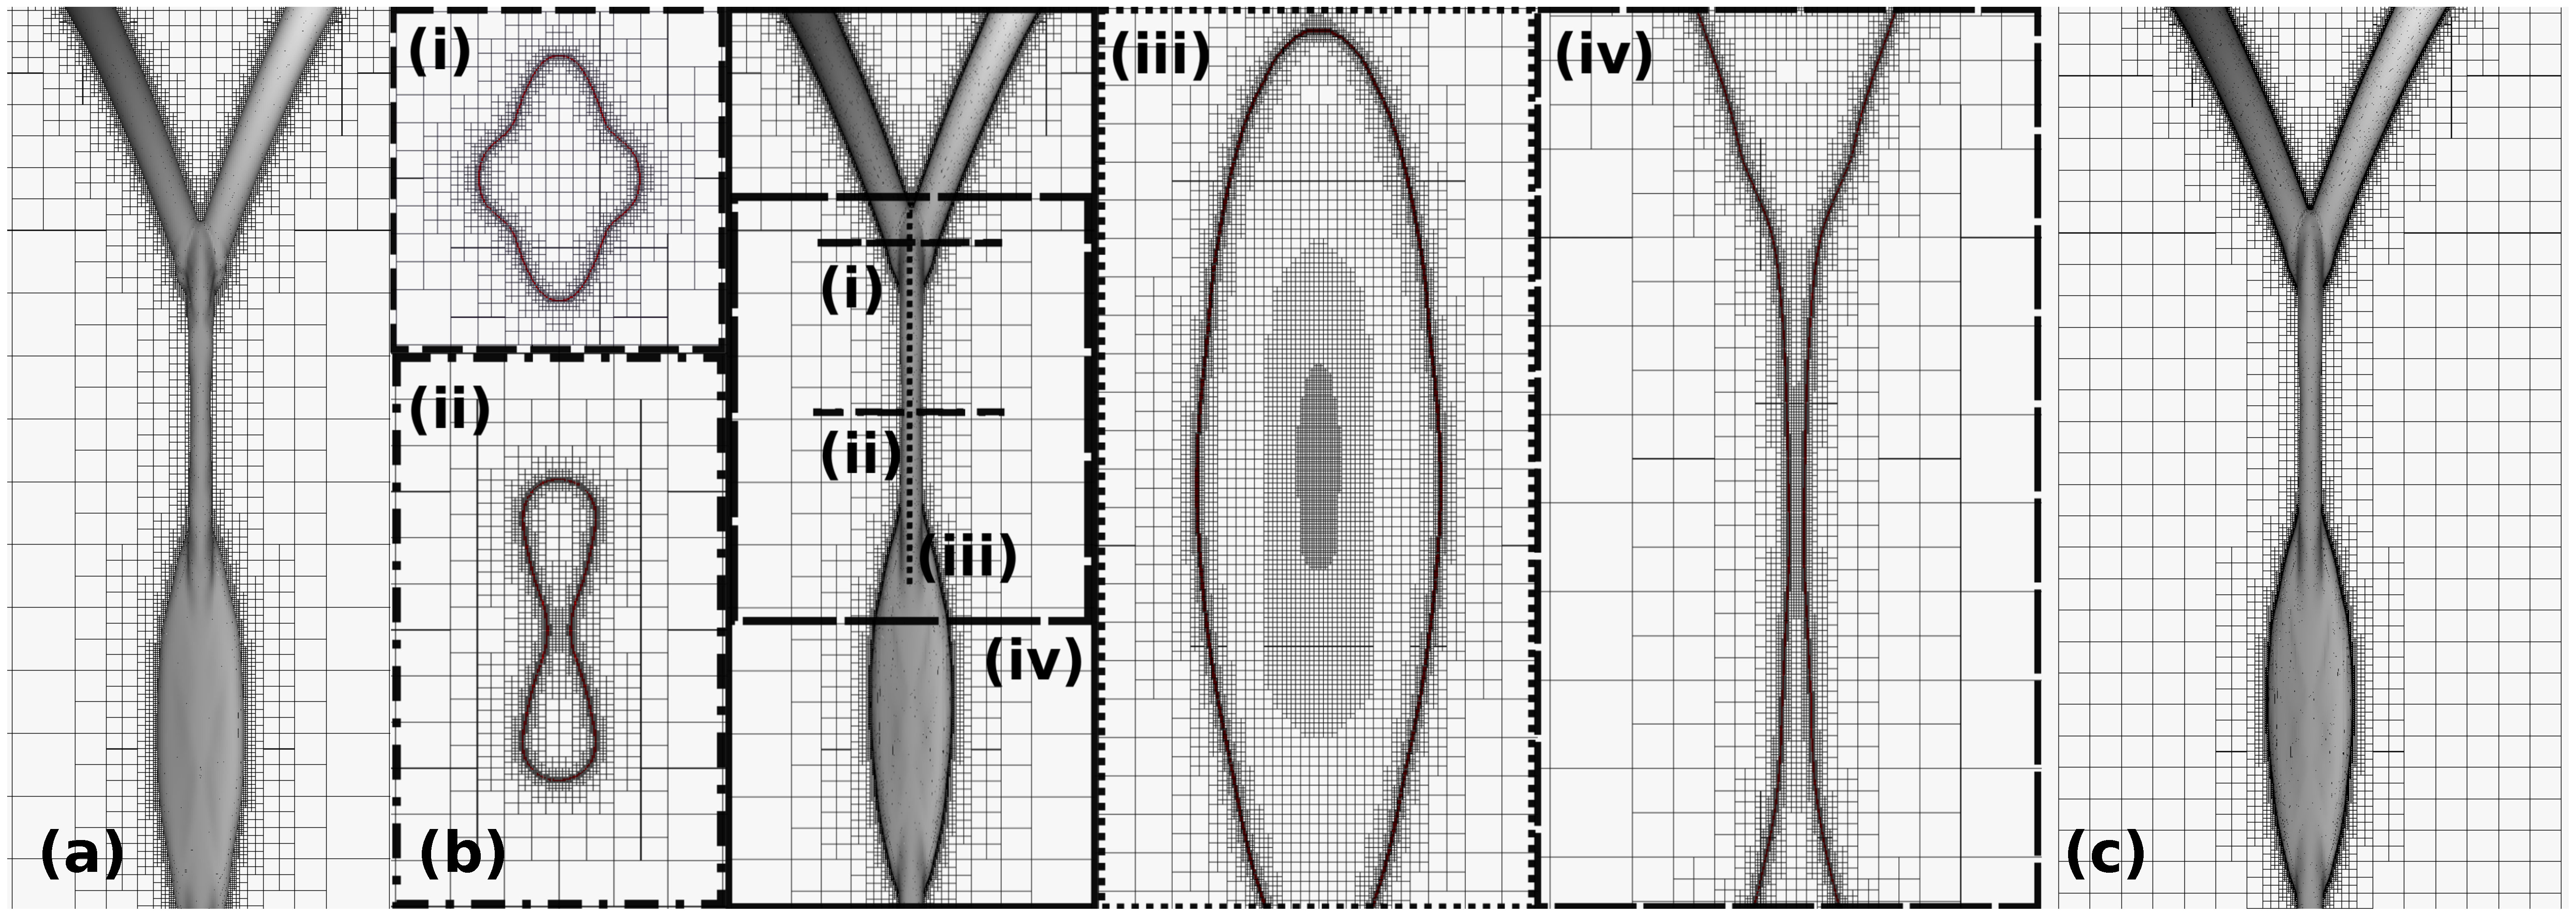
\includegraphics[width=\linewidth]{figGIS}
	\caption{Representation of the Adaptive Mesh Refinement (AMR) technique used by Gerris, the grid is finest at the interface of the two phases. Flow parameters used for Grid Independence Study (GIS) are $\alpha = 30\degree$, $Fr = 2$, $Bo = 3.4$ and $Re/Fr = 1100$, with $d_j/\delta l$ = (a) 51.2,(b) 102.4 and (c) 204.8. Sub-figures in (b) show mesh refinement at different sections of the structure (i) YZ plane at the point of collision of the jets, (ii) XZ plane of the midsection of the first link, (iii) XZ plane view of the first link and (iv) XY plane view of the first link, where the minimum thickness can be clearly identified immediately upstream of the second collision.}
	\label{Figure::GISfigures}
\end{figure*}
Sensitivity to the mesh refinement is analyzed in this section along with validation of the numerical results. Gerris uses an adaptive octree mode of refinement as illustrated in Figure~\ref{Figure::GISfigures}. It is necessary to capture the smallest features of the flow, in this case, the thickness of the liquid sheet. The multi-level grid structure adapts itself according to the gradient of the tracer $\Psi$, which implies that the structured octree mesh is finest at the interface between the two fluids. \cite{hasson1964thickness} gave a simple expression to quantify the thickness of the liquid sheet which takes the form of Equation~\ref{Equation::hrHassaon}.
\begin{equation}\label{Equation::hrHassaon}
\frac{hr}{d_j^2} = 	\frac{1}{4}\frac{sin^3\alpha}{(1-cos\theta\:cos\alpha)^2}
\end{equation}
\begin{figure}
	\centering
	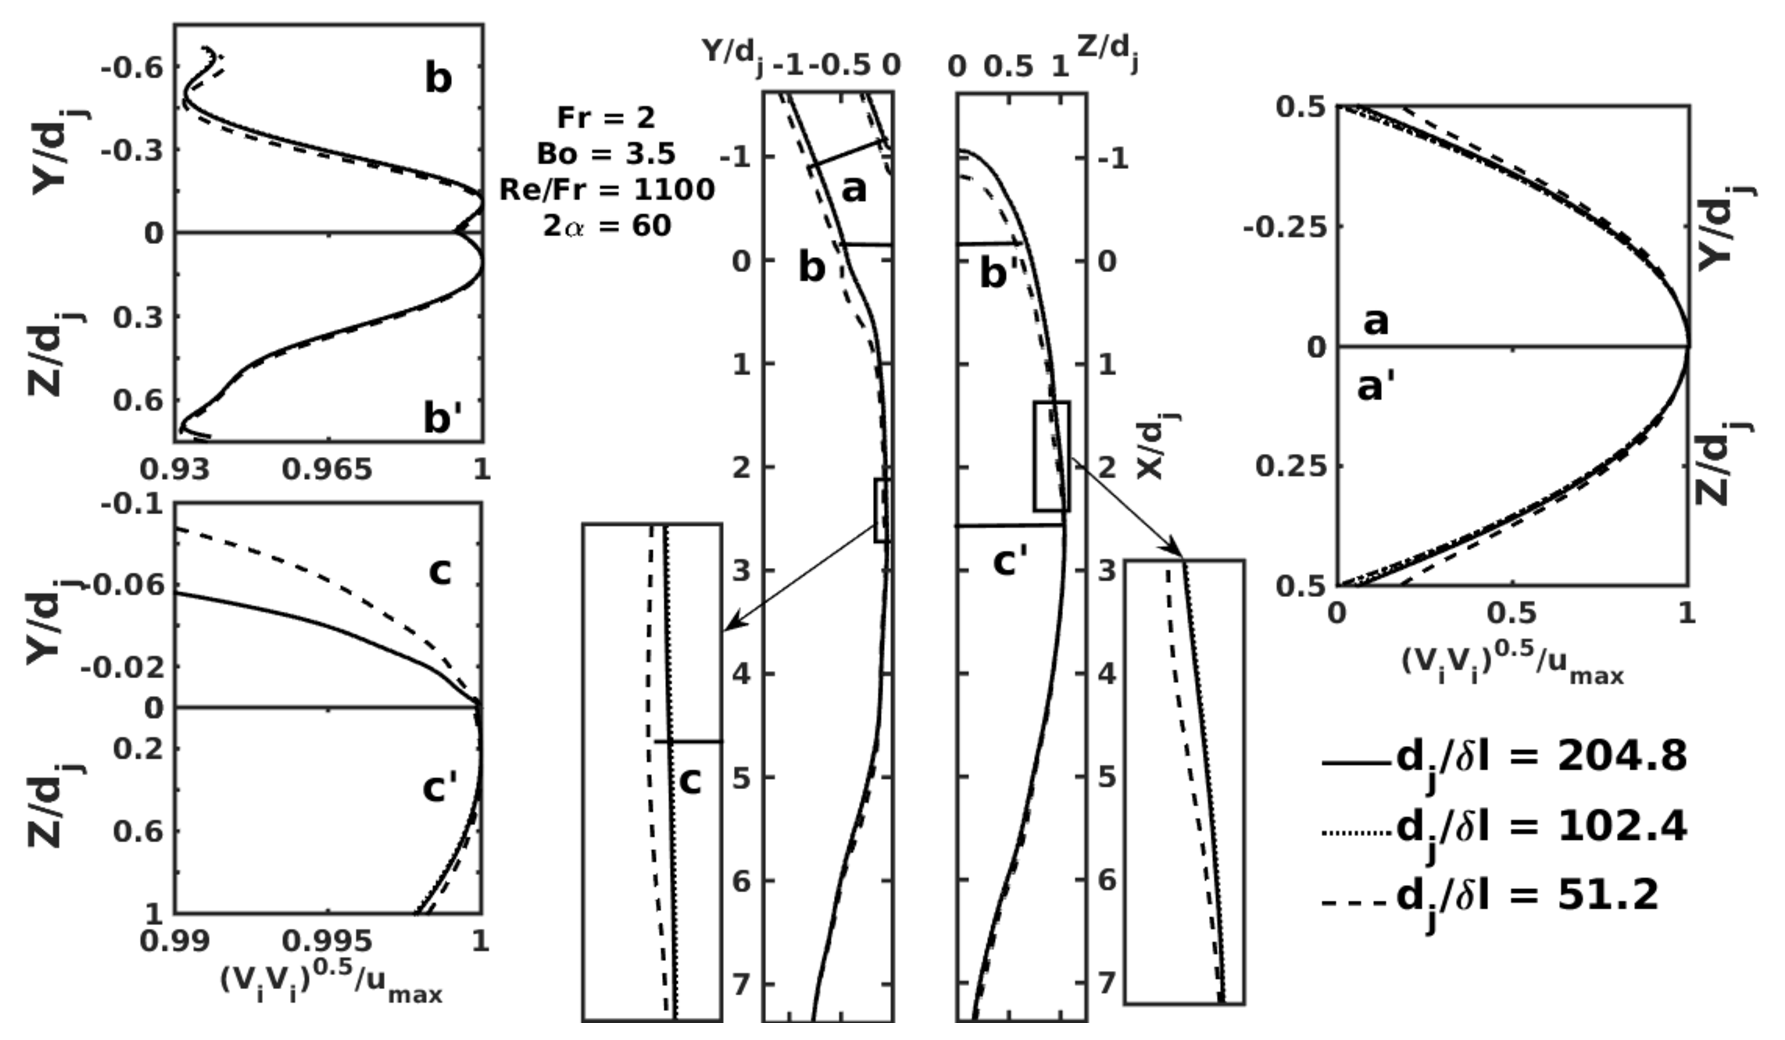
\includegraphics[width=\linewidth]{gis}
	\caption{Illustration of the results of Mesh Sensitivity Analysis for a typical chain structure, having $\alpha = 30\degree$, $Fr = 2$, $Bo = 3.4$ and $Re/Fr = 1100$. The volume fraction $\left(\Psi\right)$ contours (main figures and magnified in inset) show saturation on increasing the refinement from $d_j/\delta l$ = 102.4 to 204.8. Velocity profiles at different sections across the chain structure are shown for (a-a$'$) Inside the liquid jet, (b-b$'$) Just downstream of the point of collision  and (c-c$'$) At the plane of maximum extent of the liquid sheet.}
	\label{Figure::GISplots}
\end{figure}
Although the minimum of Equation~\ref{Equation::hrHassaon} occurs at $\theta \to \pi$, it must be noted that the decrement in thickness is more because of the increase in radial distance downstream of the first collision point $\left(h \propto \frac{1}{r}\right)$, which is maximum near low azimuthal angles (Figure~\ref{Figure::GISfigures}(b - iv)), just upstream of the second collision point. This happens because the fluid velocity increases as the gravitational potential is converted to kinetic energy and the thickness decreases to keep the mass flow rate constant. An order of magnitude analysis reveals that $\frac{hr}{d_j^2} \sim 1$ for the minimum thickness at $2\alpha = \frac{\pi}{2}$ in the range of our numerical simulations. Therefore, $\frac{d_j}{\delta l} \sim 10\frac{r_{max}}{d_j}$ can be used as an imperative starting point for the grid independence study. The factor of 10 is included to have at least 10 grid points across the smallest length scale for the structure to be fully resolved \citep{ling2015multiscale}, else the sheet thickness will be equal to the minimum grid size and the sheet would break at the cost of being unresolved \citep{chen2013high}.
\begin{table}[]
	\caption{Performance data of the processors used for simulations to determine the refinement level in the Grid Independence Study. The simulations are done using four Intel Core i7-6500U CPU having clock speed of 2.5GHz each and 8 GB RAM.}
	\label{Table::cpu}
	\centering
	\begin{tabular}{@{}cc@{}}
		\hline
		\begin{tabular}[c]{@{}c@{}} $\: \: \: \: \: \: \: \: \: \left(\frac{d_j}{\delta l}\right)_{max}$ \end{tabular} & \begin{tabular}[c]{@{}c@{}} $\: \: \: \: \: \: \: \: \: \left(\frac{t_{CPU}}{t_{actual}}\right)$ \\ $\: \: \: \: \: \: \: \: \:$(days/s) \end{tabular}\\ \hline
		51.2 & $\sim 20$\\
		102.4 & $\sim 28$ \\	
		204.8 & $\sim 60$ \\	\hline
	\end{tabular}
\end{table}
\begin{figure}
	\centering
	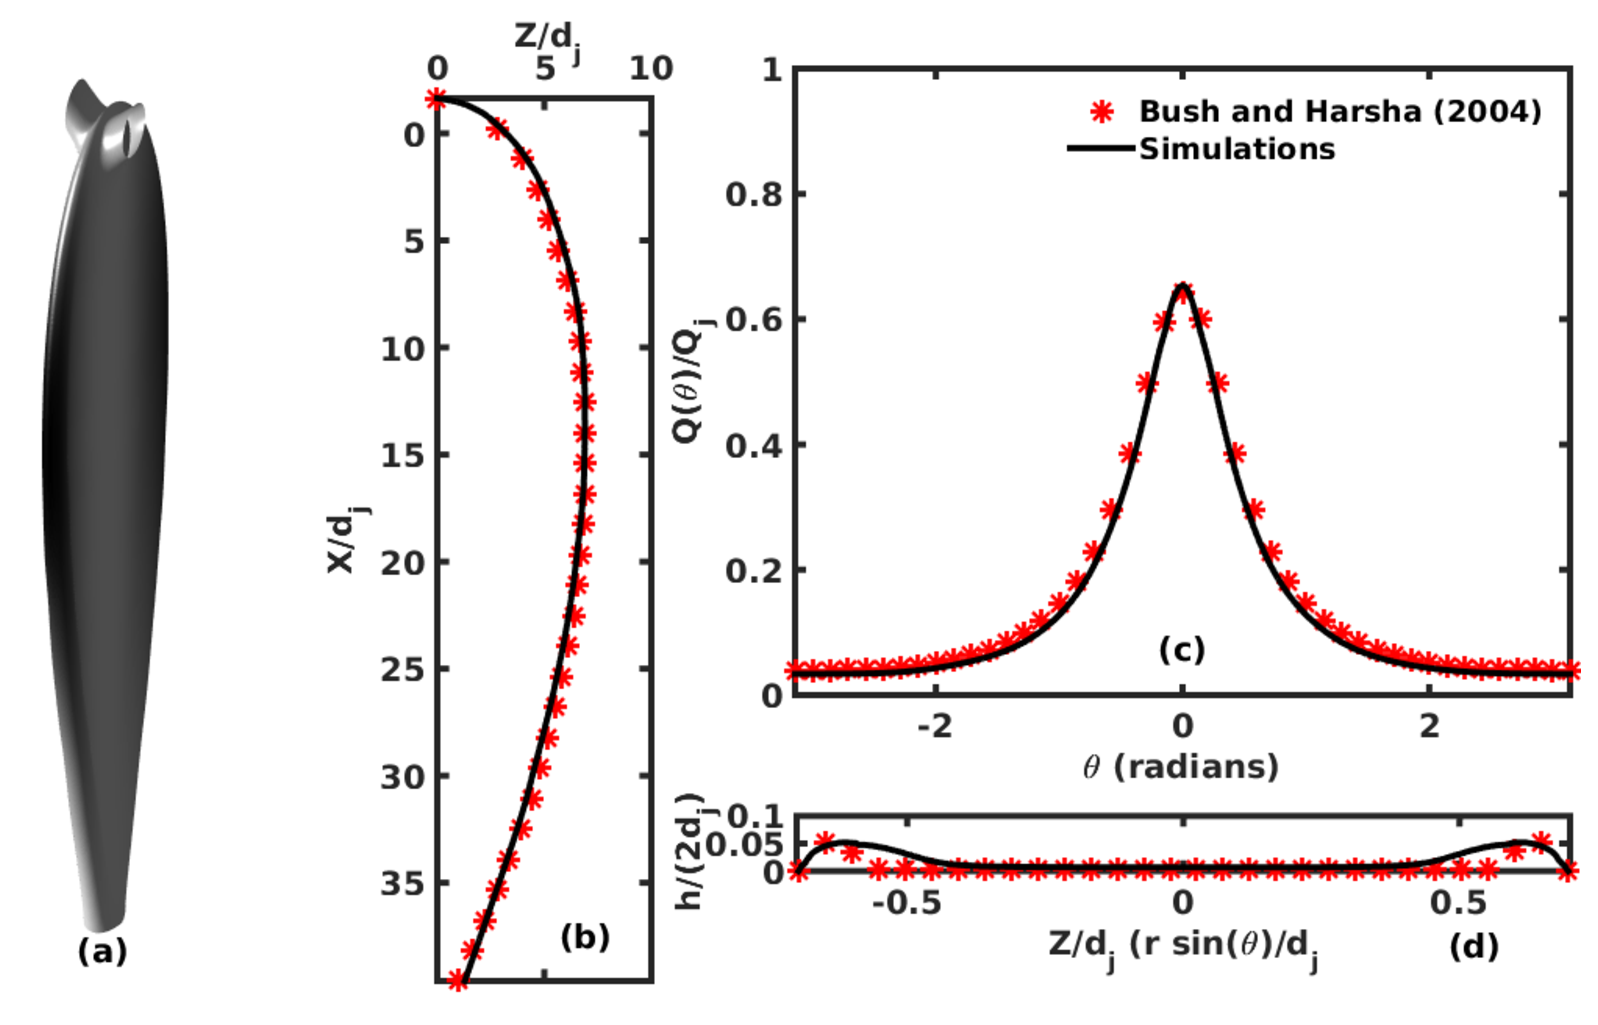
\includegraphics[width=\linewidth]{validation}
	\caption{Validation of the numerical model employed with the experimental results obtained by \cite{bush2004collision}: (a) The iso-surface volume fraction contour showing the first link of the chain, (b) Volume fraction contour in the X-Z plane at y = 0 showing the boundary of the first link, (c) Variation of the liquid volume flux ($Q(\theta)$, non-dimensionalized with the volume flow rate of the jet, $Q_j$) and (d) Thickness profile of the liquid sheet obtained at a distance of 17.25$d_j$ from the point of the first collision.}
	\label{Figure::validation}
\end{figure}
Figure~\ref{Figure::GISplots} gives a representative case employed for the grid independence study. Applying above discussed arguments, $\frac{d_j}{\delta l} \sim 70$ (Figure~\ref{Figure::GISfigures}(a)) should be ideal for the simulations. It can be  clearly seen that the variations in the results such as the contour of the tracer (volume fraction) and velocity profiles at different locations downstream of the collision point, saturate if the refinement is increased from $\frac{d_j}{\delta l} = 102.4$ (Figure~\ref{Figure::GISfigures}(b)) to $204.8$ (Figure~\ref{Figure::GISfigures}(c)). Moreover, the later requires more computational power and time (Table~\ref{Table::cpu}). Therefore, a refinement level of $\frac{d_j}{\delta l} = 102.4$ is employed for this case. A similar analysis is carried out for all the cases reported in the present study initiated with $\frac{d_j}{\delta l} = 10\frac{r_{max}}{d_j}$, with $r_{max} = 10d_j$. If the sheet is still not fully resolved or the maximum radial extent of a given link goes higher that $10d_j$, the refinement level is increased.\\
Next, we use the experimental results obtained by \cite{bush2004collision} to validate the employed numerical model. Figure~\ref{Figure::validation} presents a description of the results of this test. The first link of the chain structure formed is illustrated in Figure~\ref{Figure::validation}(a), with matching between the experimentally obtained boundary of the link and the contour generated from numerical simulations shown in Figure~\ref{Figure::validation}(b). Making use of the fact that their experiments led to a supercritical (greater than the capillary wave speed) sheet speeds, \cite{bush2004collision} were able to construct the variation of the liquid volume flux $\left(Q(\theta) = \frac{dQ}{d\theta} = uhr\right)$ inside the sheet by scanning across the sheet and collecting liquid through a fine opening. Figure~\ref{Figure::validation}(c) shows the variation of the liquid flux with the azimuthal angle inside the sheet along with the reconstruction of the flux profile by our numerical simulation. Moreover, the thickness of the liquid sheet is one of the major attributes that must be predicted by the numerical simulations. Figure~\ref{Figure::validation}(d) gives a one-to-one correspondence between the thickness profile obtained at a distance of 17.25$d_j$ from the point of the first collision. One can clearly observe the presence of a thick rim at the periphery of the sheet. Next, the transient process of impact of the liquid jets is analyzed, followed by the kinematic description of the flow inside the sheet using the velocity profile analysis and an outlook of the streamlines. 
\section{Formation of the chain}
\lipsum[1]
\subsection{Towards the steady state}
\lipsum[1]
\begin{figure}
	\centering
	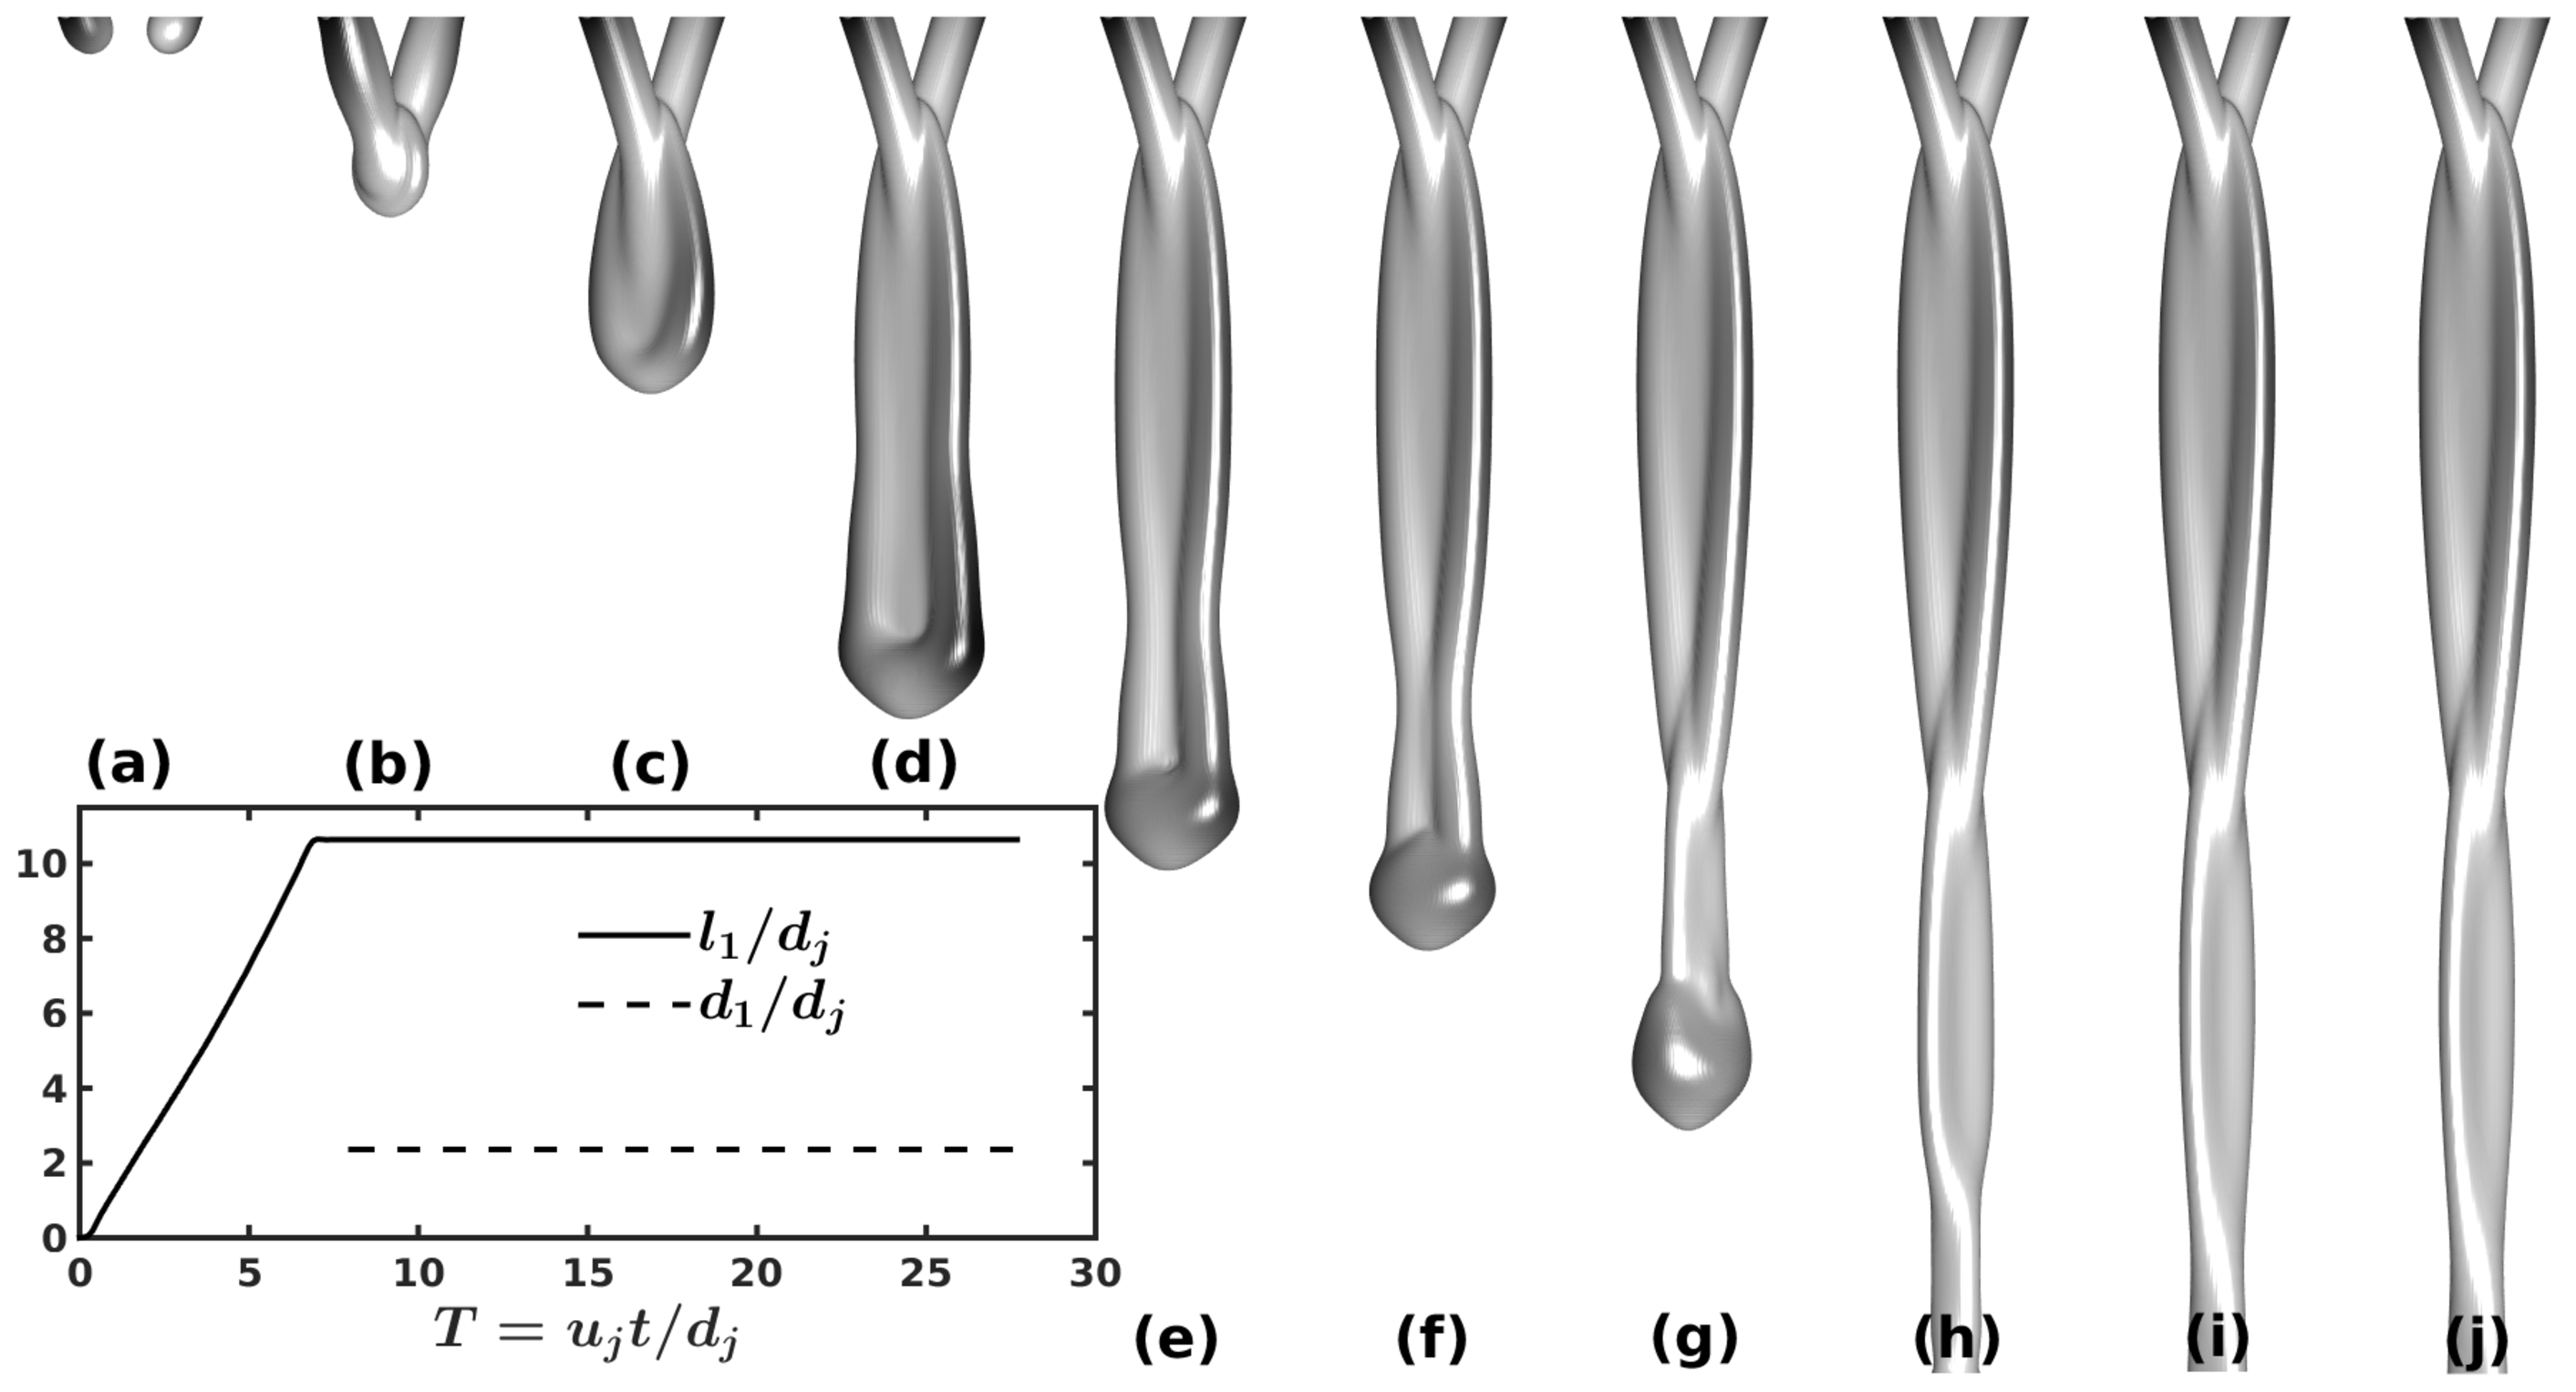
\includegraphics[width=\linewidth]{fig0}
	\caption{Transition to the steady state fluid-links chain formed by collision of laminar jets. The figure illustrates the transient period through the temporal advancement from (a) pre-collision symmetric jets to $T (\frac{u_jt}{d_j}) = $ (b) 1.5, (c) 4, (d) 5, (e) 5.5, (f) 6.5, (g) 8.5, (h) 16.5, (i) and (j) 20}
	\label{Figure::transient}
\end{figure}
\lipsum
\section{Velocity Field Description}
\lipsum[1]
\subsection{First Link Velocity Field}
\lipsum
\subsection{Overall streamlines}
\lipsum[1]
\begin{figure}
	\centering
	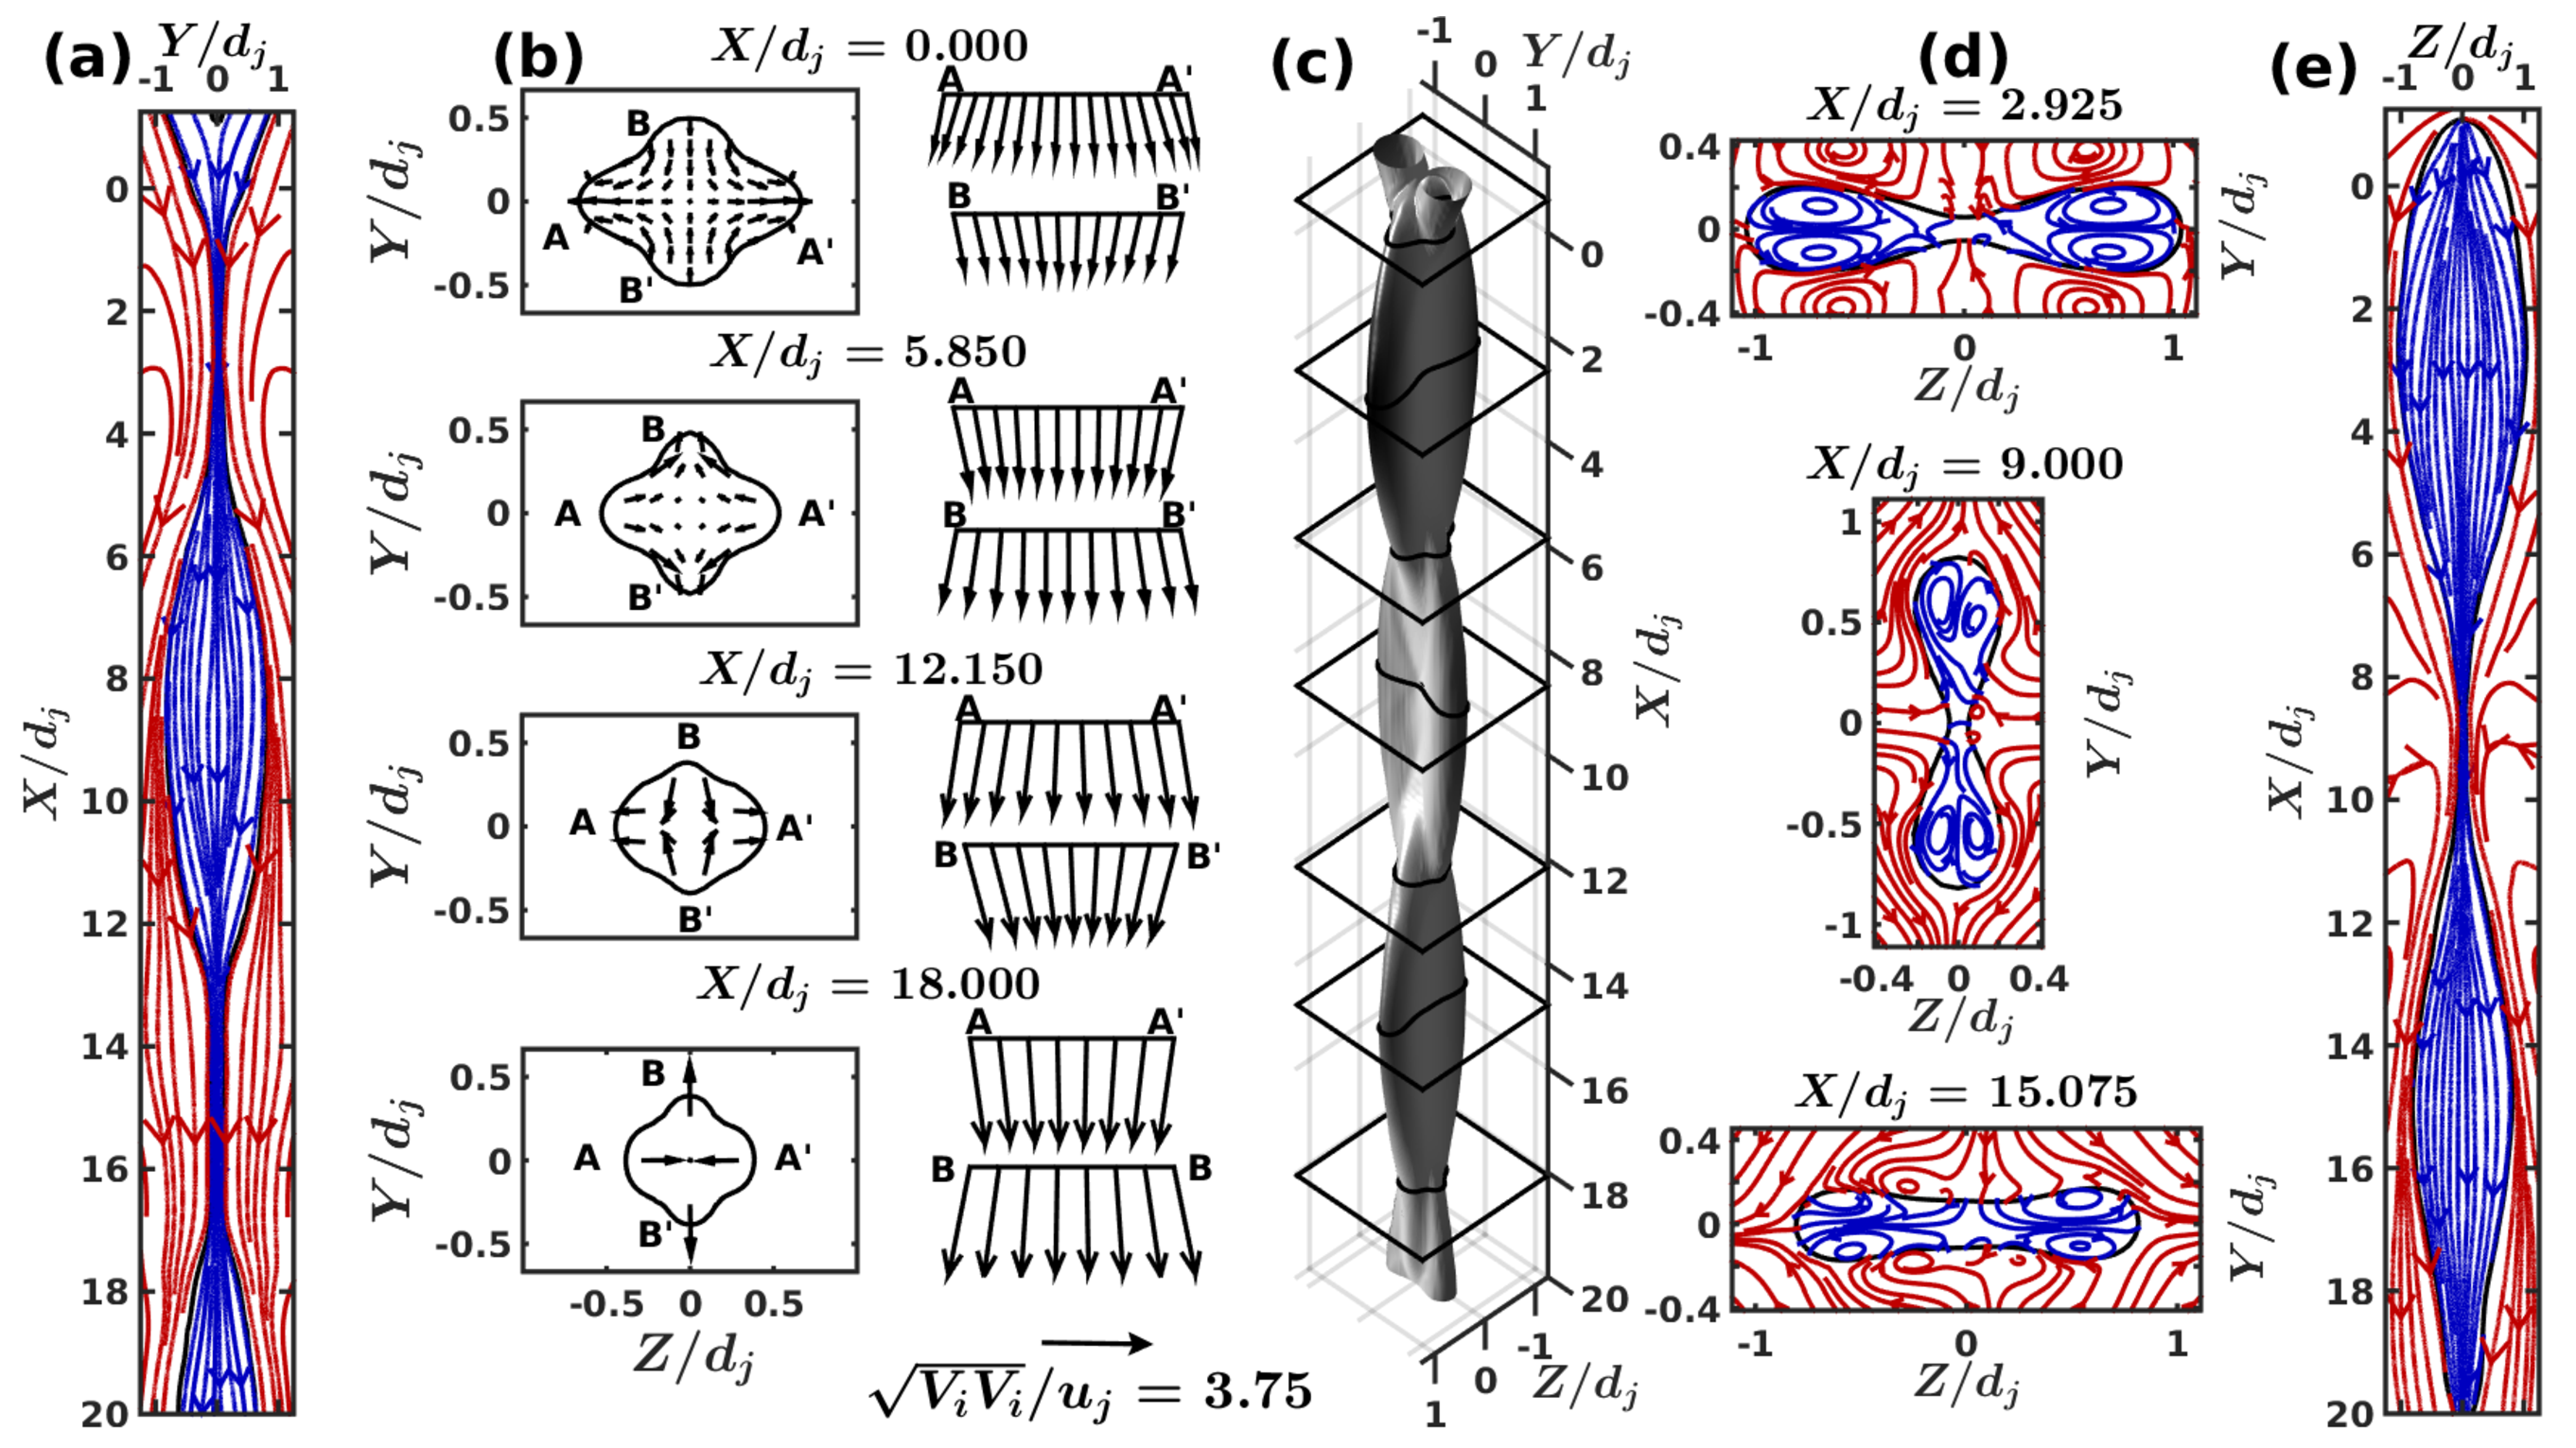
\includegraphics[width=\linewidth]{streamlinesDetails}
	\caption{}
	\label{Figure::streamDetails}
\end{figure}
\lipsum
\subsection{Twisting of streamlines}
\lipsum[1]
\begin{figure}
	\centering
	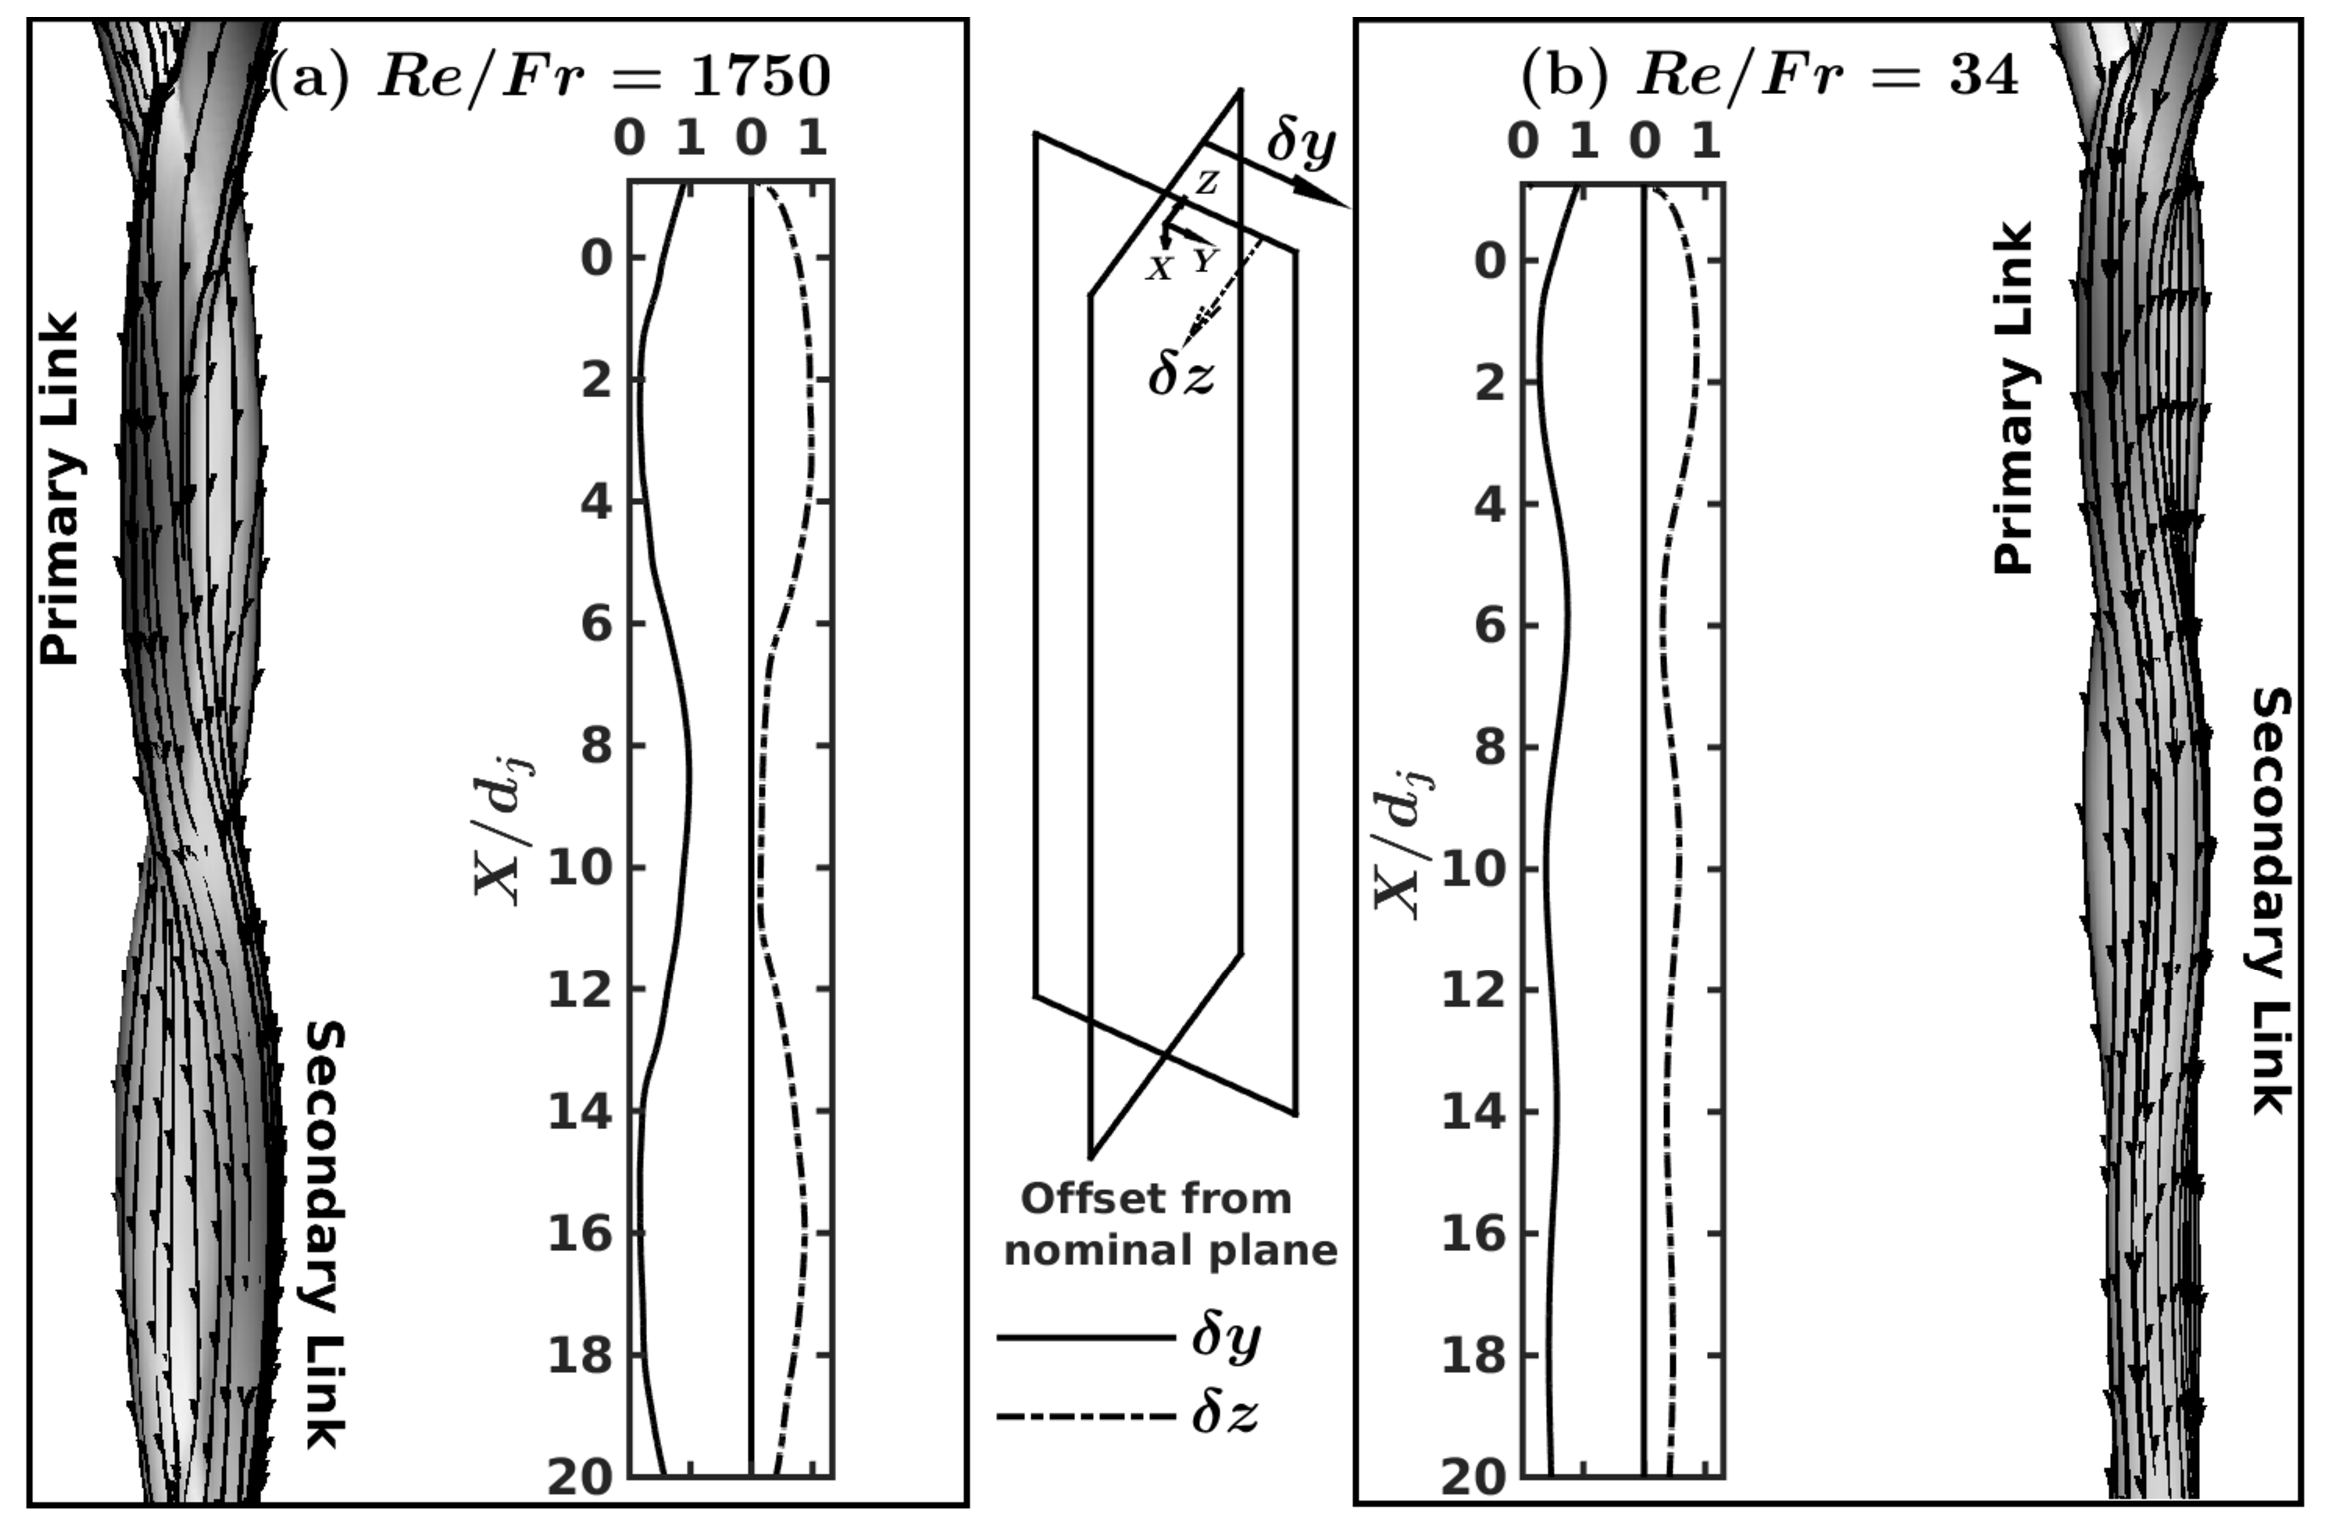
\includegraphics[width=\linewidth]{fig1}
	\caption{}
	\label{Figure::stream}
\end{figure}
\lipsum[1]
\section{Parametric variations}
\subsection{Phase contours for different cases}
\lipsum[1]
\begin{figure*}
	\centering
	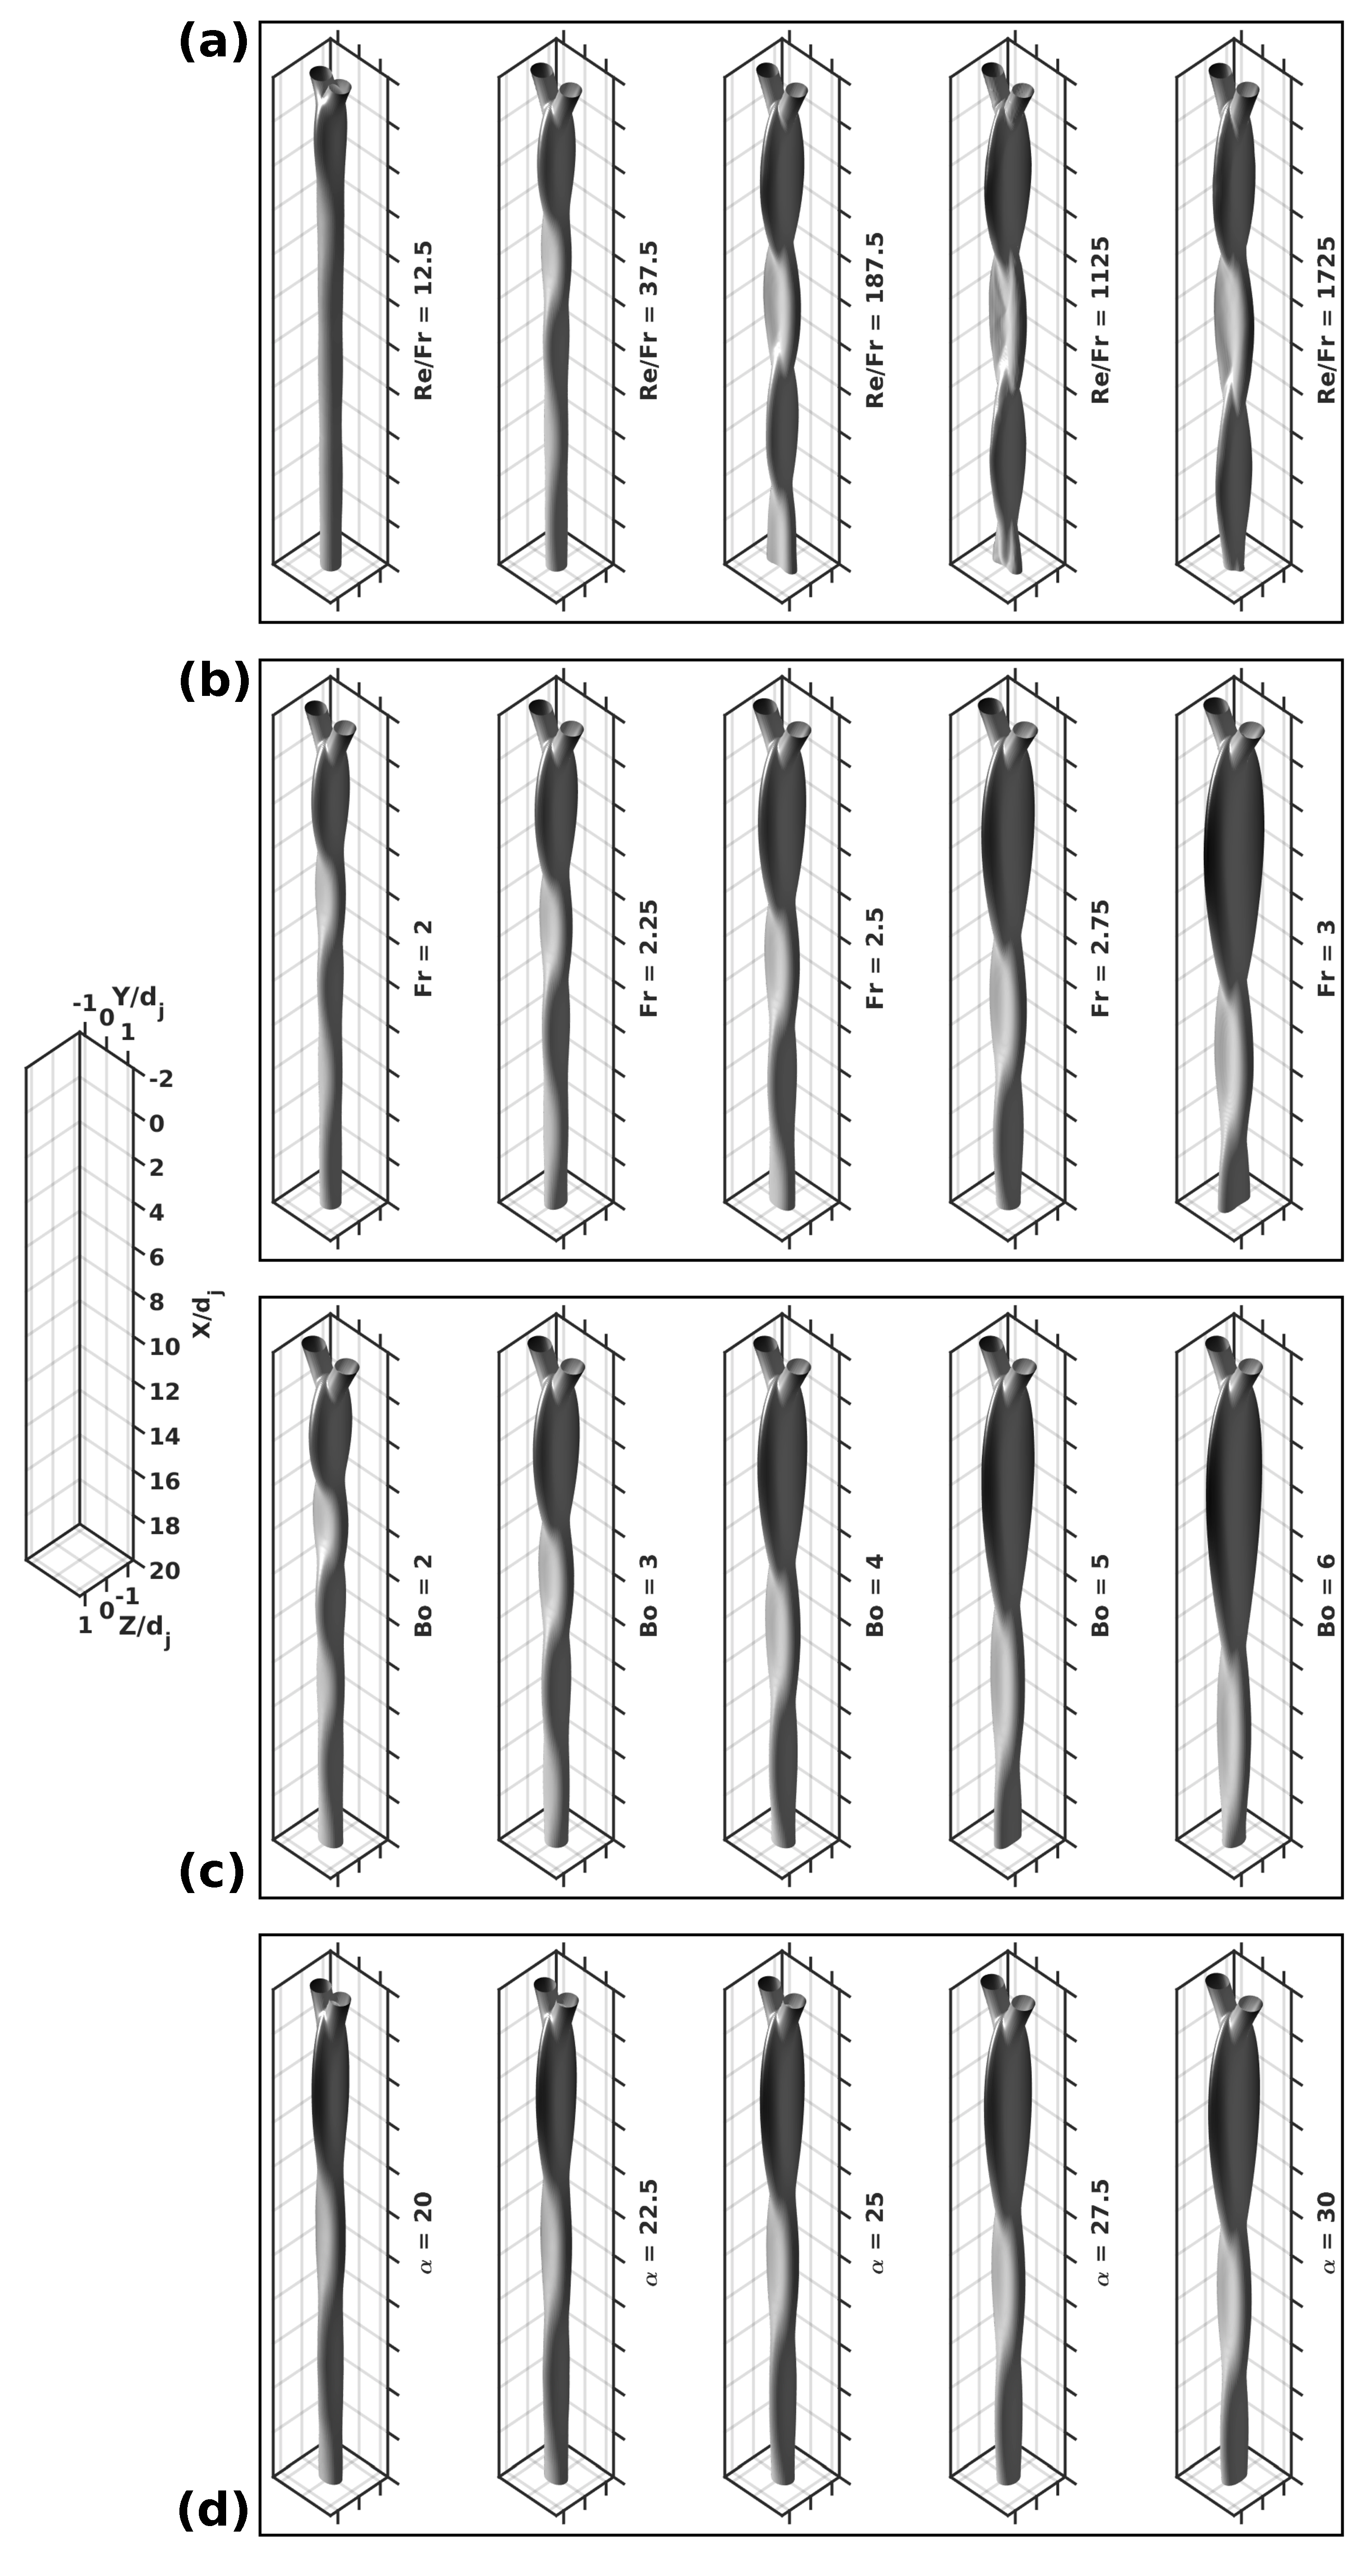
\includegraphics[width=\linewidth]{phaseContours}
	\caption{}
	\label{Figure::phaseContours}
\end{figure*}
\lipsum[1]
\subsection{First link phase contour}
\begin{figure}
	\centering
	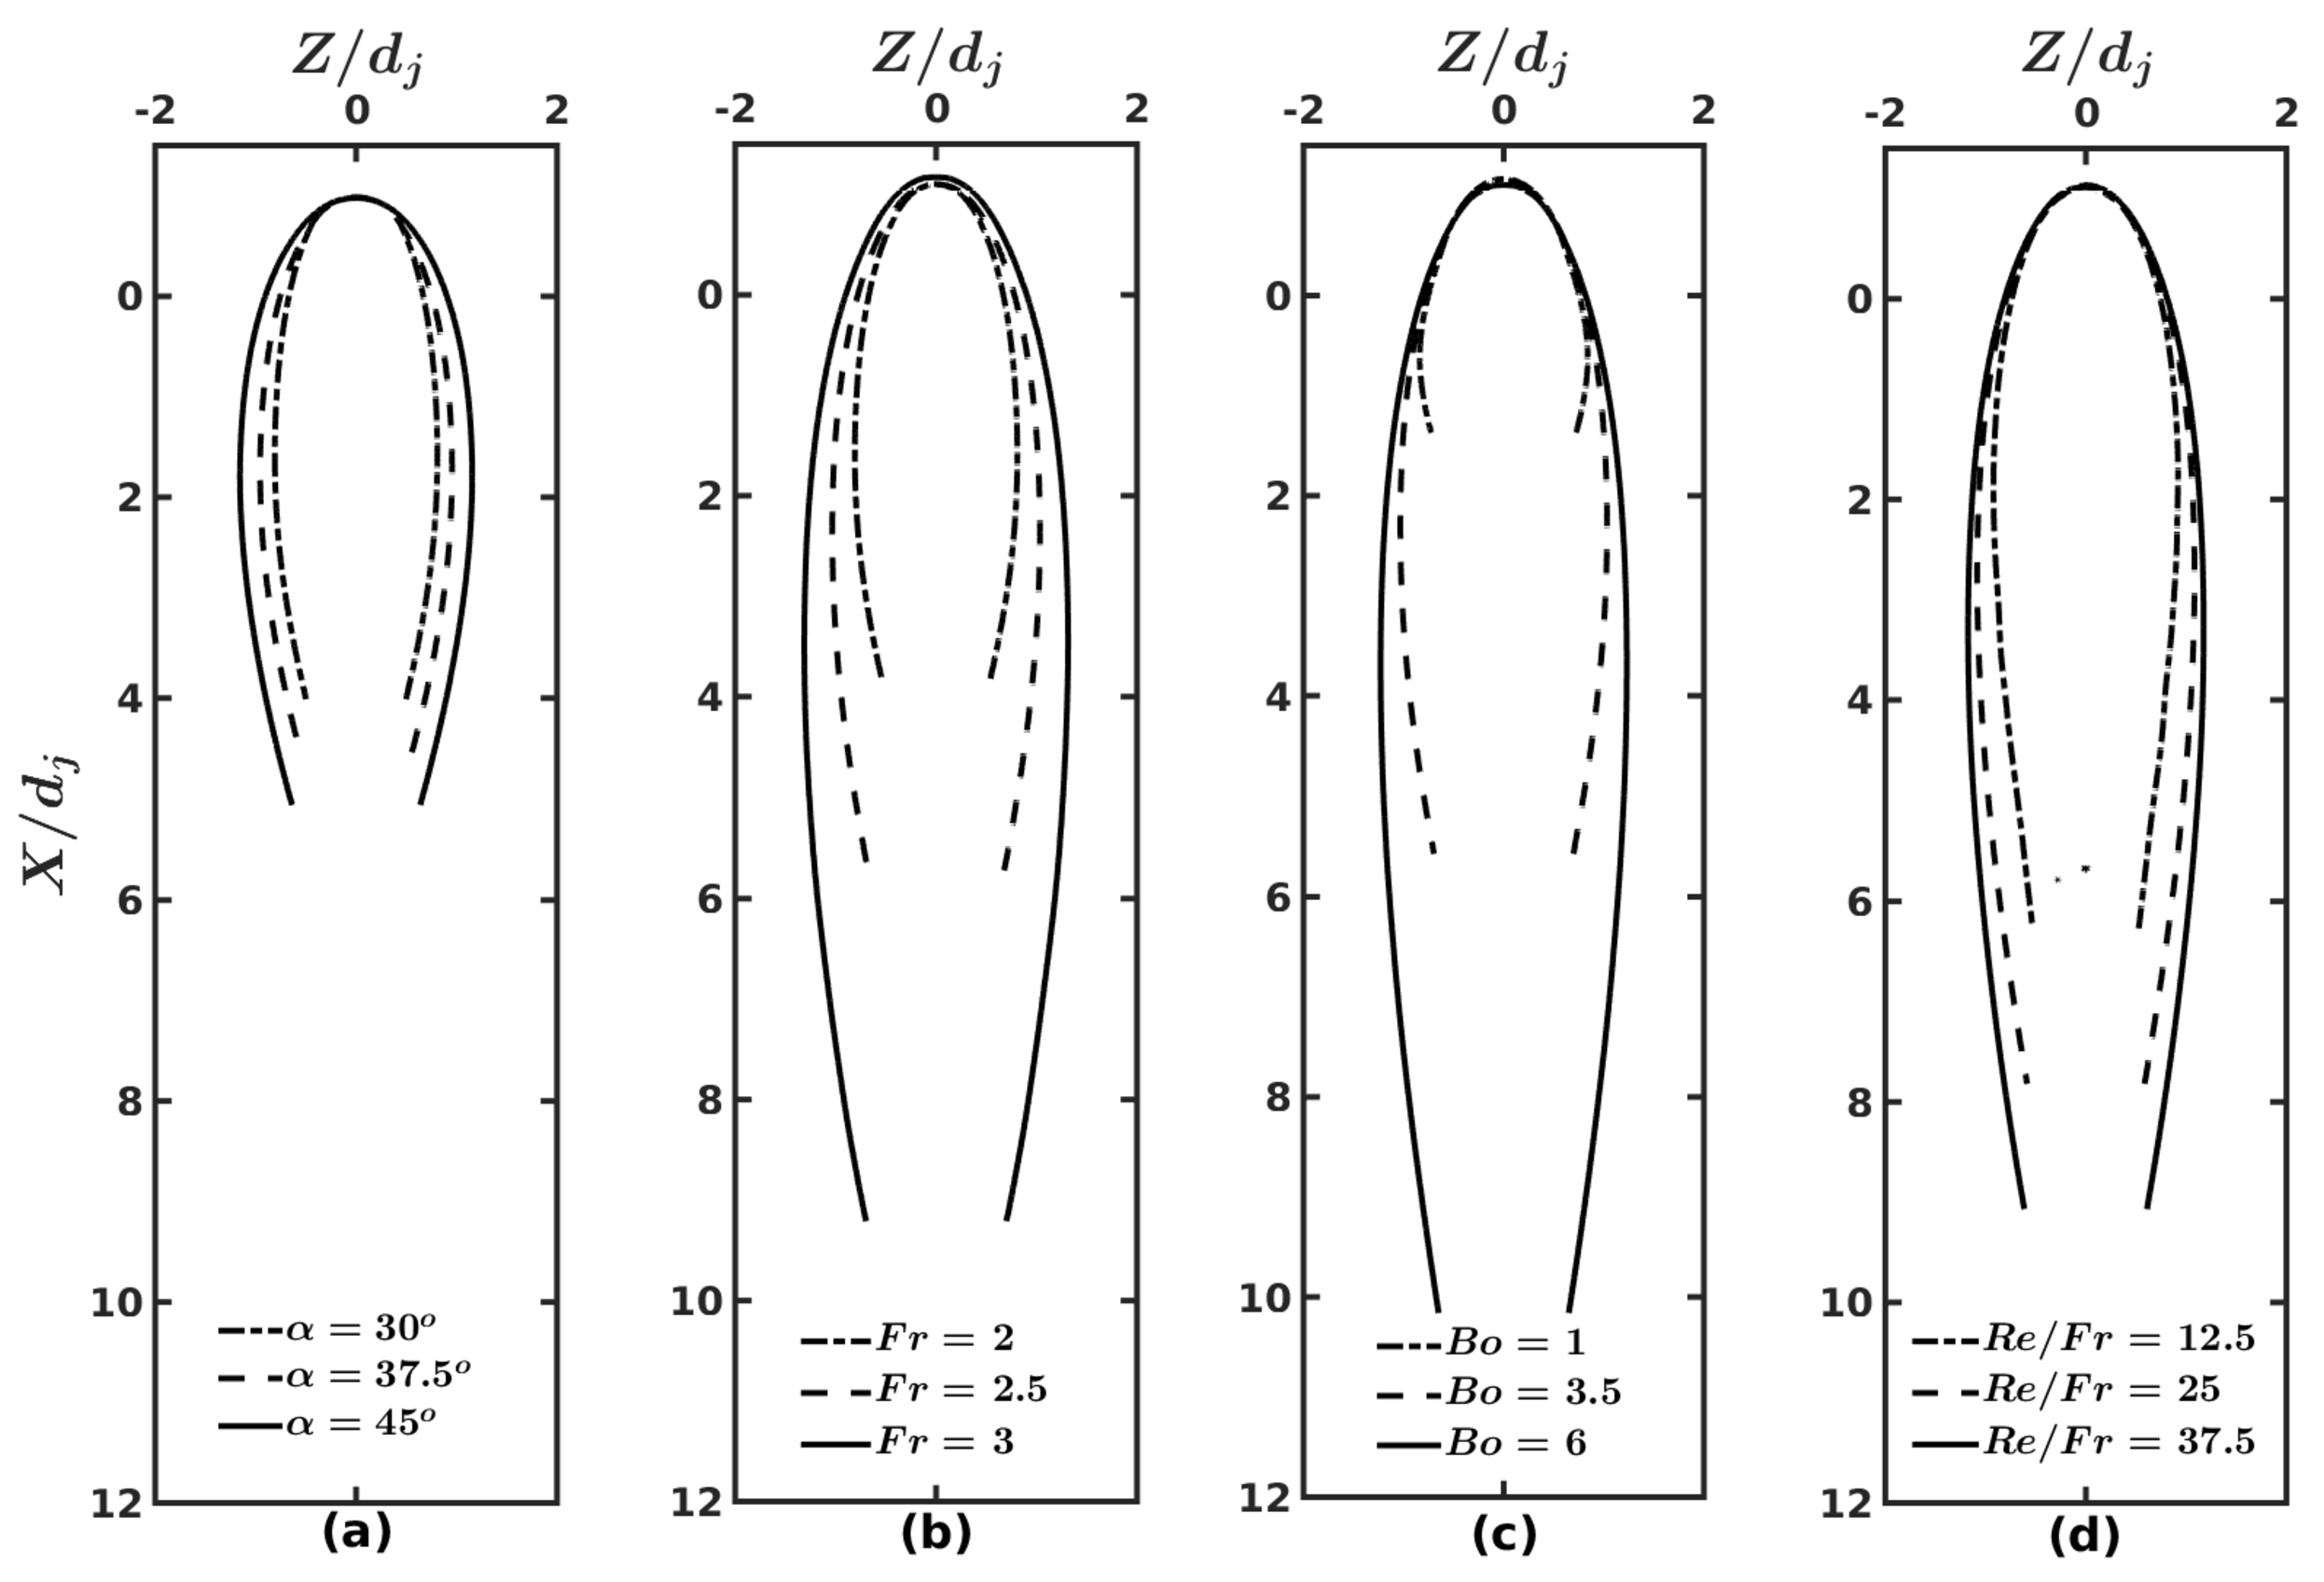
\includegraphics[width=\linewidth]{finalContour}
	\caption{}
	\label{Figure::finalContours}
\end{figure}
\lipsum
\section{Predicting the shape of the first link}
\lipsum[1]
\subsection{Co-relation model}
\lipsum[1]
\begin{figure}[H]
	\centering
	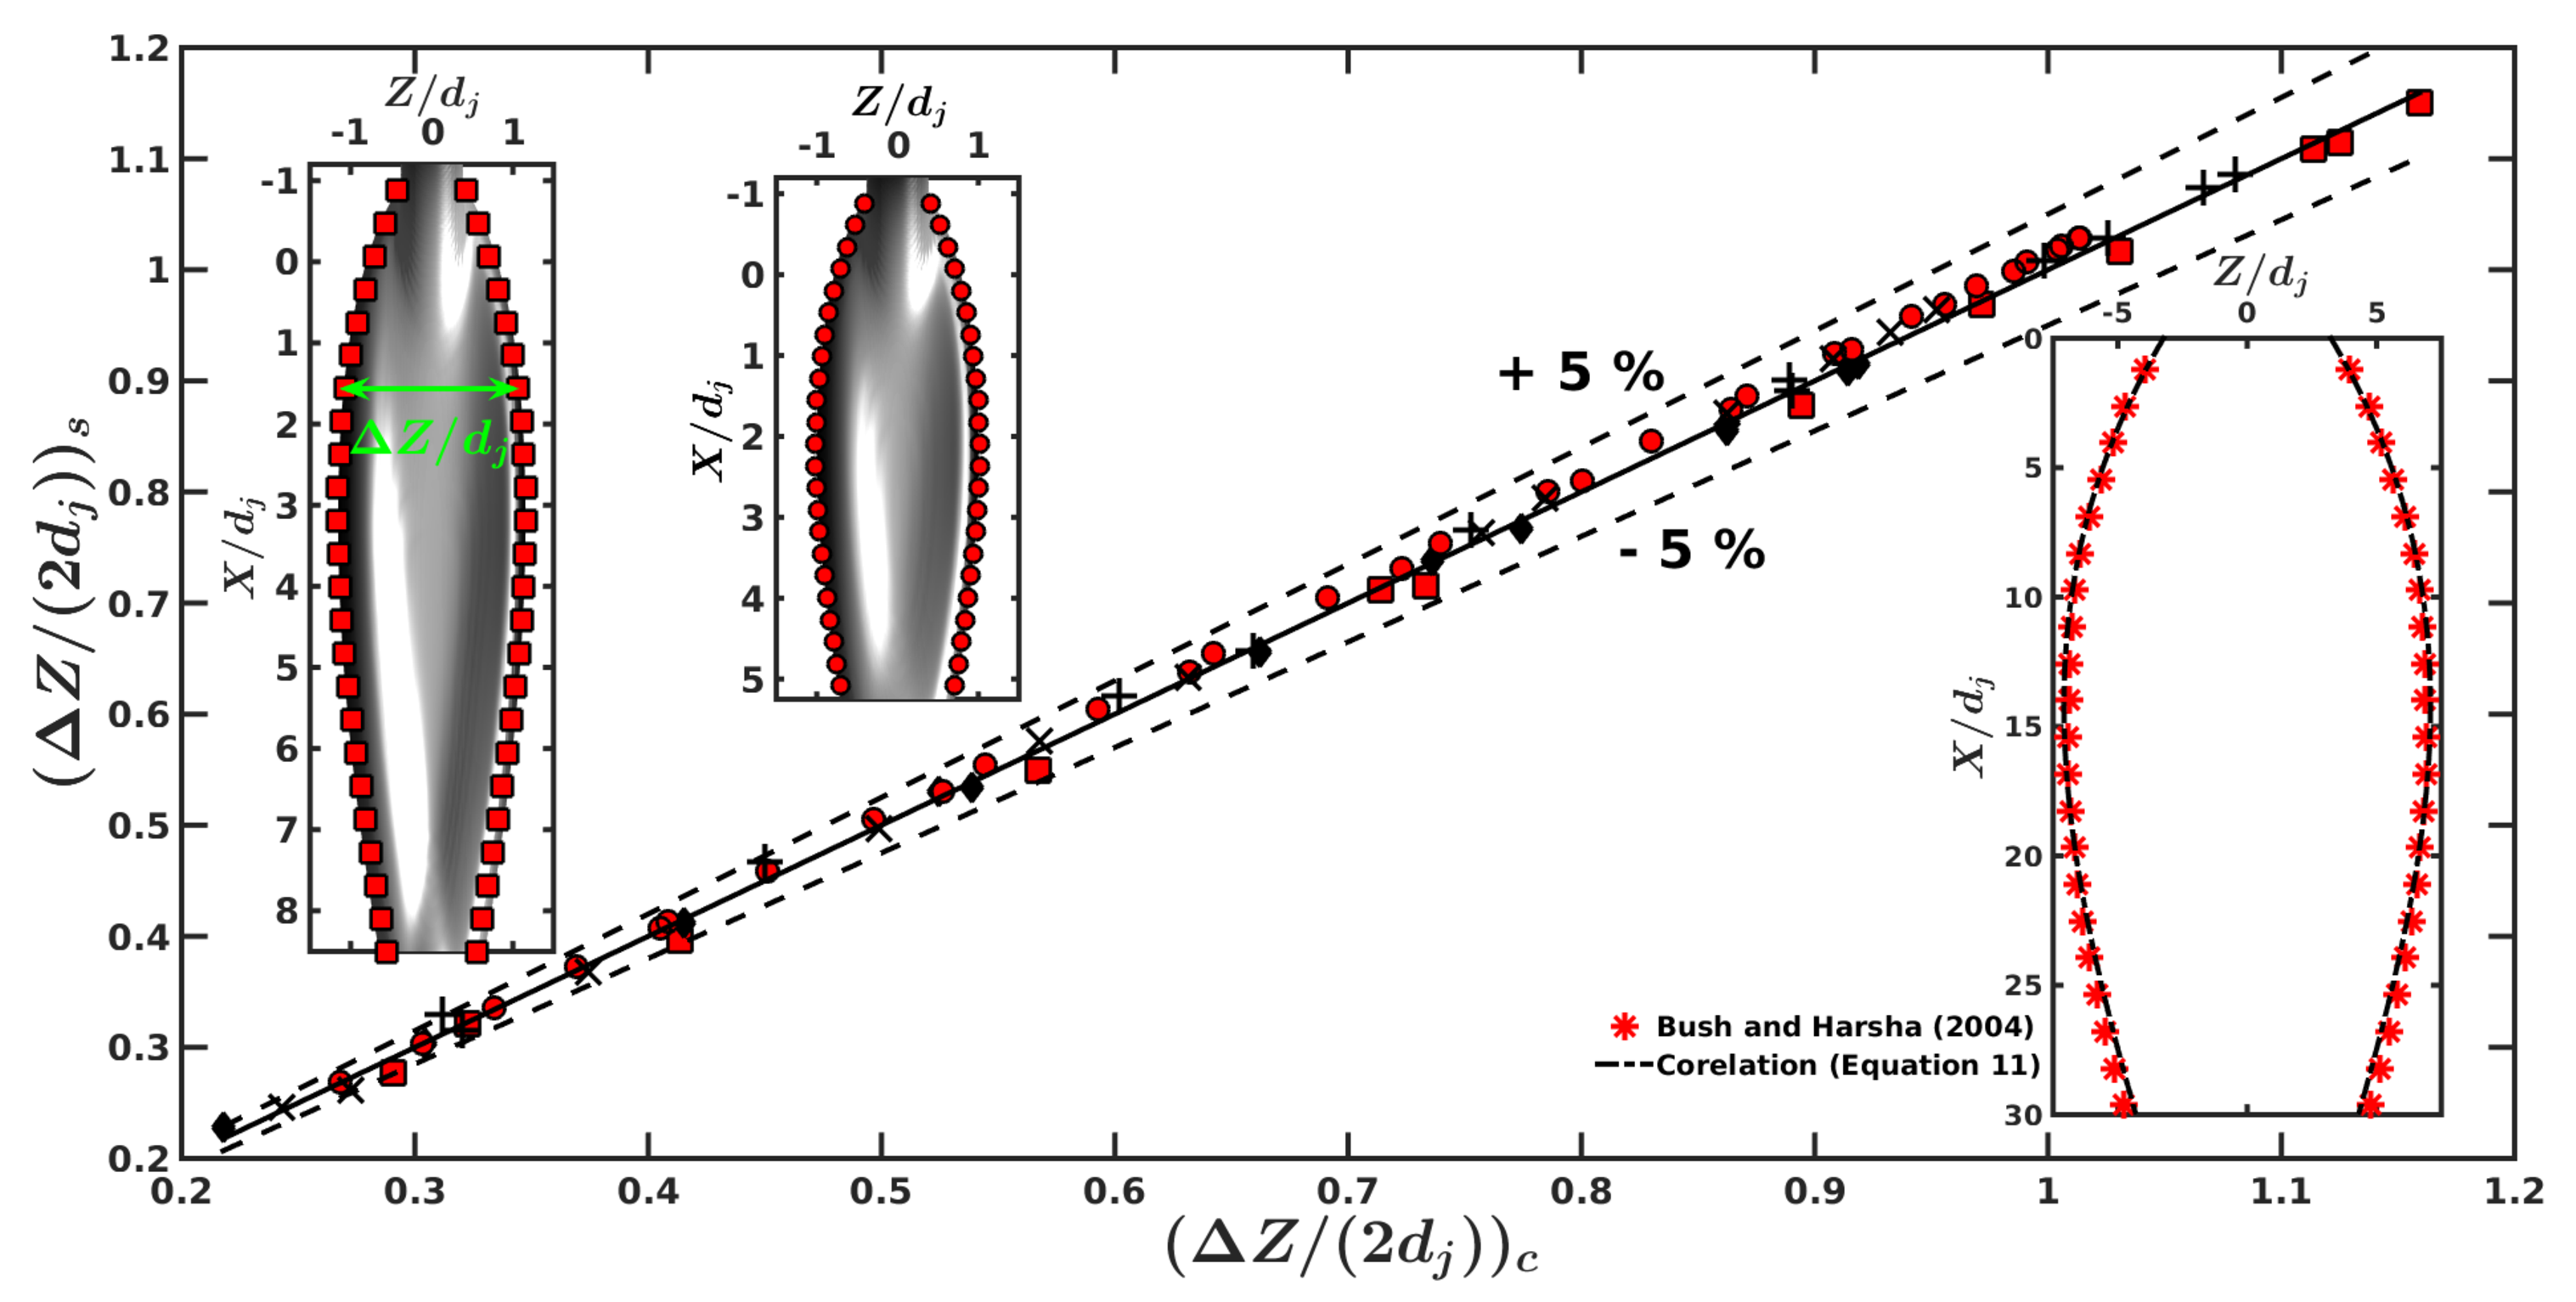
\includegraphics[width=\linewidth]{corelatehx}
	\caption{$\alpha$ = 30, $Fr$ = 2.5, $Bo$ = 5 and $Re/Fr$ = 34 (\protect\MarkerSquareRed); $\alpha$ = 30, $Fr$ = 2.5, $Bo$ = 4 and $Re/Fr$ = 34 (+); $\alpha$ = 30, $Fr$ = 2.5, $Bo$ = 2.3 and $Re/Fr$ = 20 (\protect \MarkerDiamondBlack); $\alpha$ = 25, $Fr$ = 2.5, $Bo$ = 4.57 and $Re/Fr$ = 34 ($\times$) and $\alpha$ = 30, $Fr$ = 2.5, $Bo$ = 3.75 and $Re/Fr$ = 20 (\protect \MarkerCircleRed) }
	\label{Figure::corelatehx}
\end{figure}
\lipsum
\subsection{Analytical model}
\lipsum[1]
\begin{figure}
	\centering
	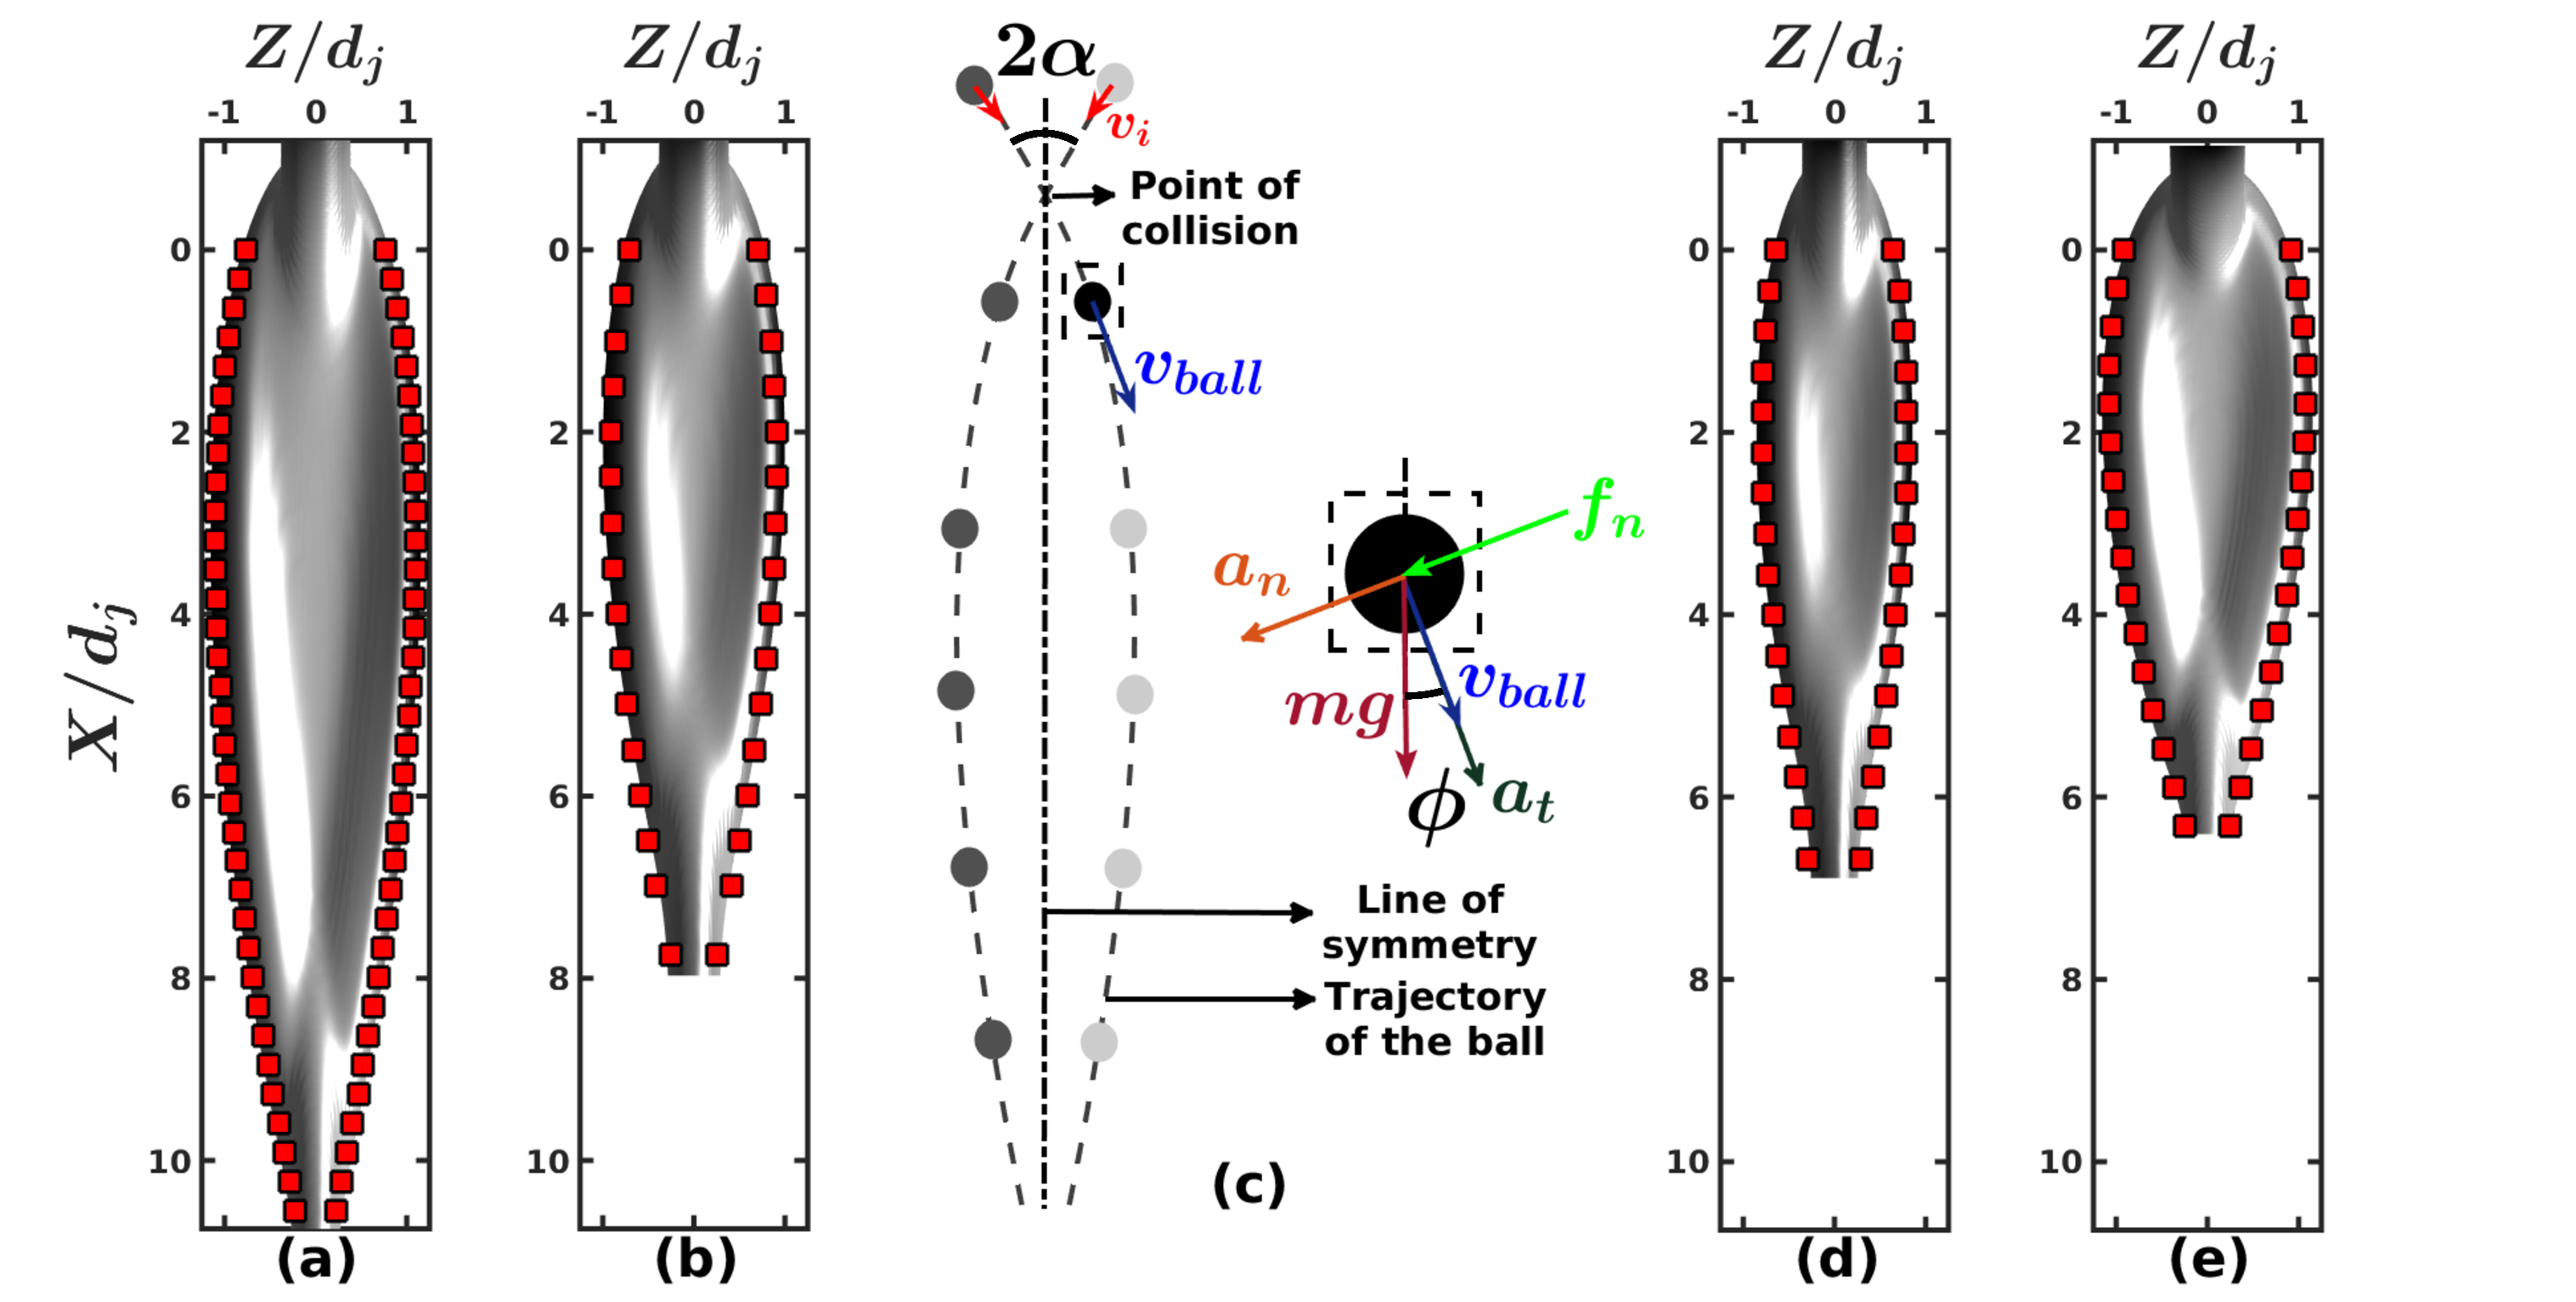
\includegraphics[width=\linewidth]{analytical}
	\caption{}
	\label{Figure::analytical}
\end{figure}
\lipsum[1]

\lipsum[1]
\section{Second - Collision}
\lipsum[1]
\subsection{Analogies for second collision}
\lipsum
\begin{figure}
	\centering
	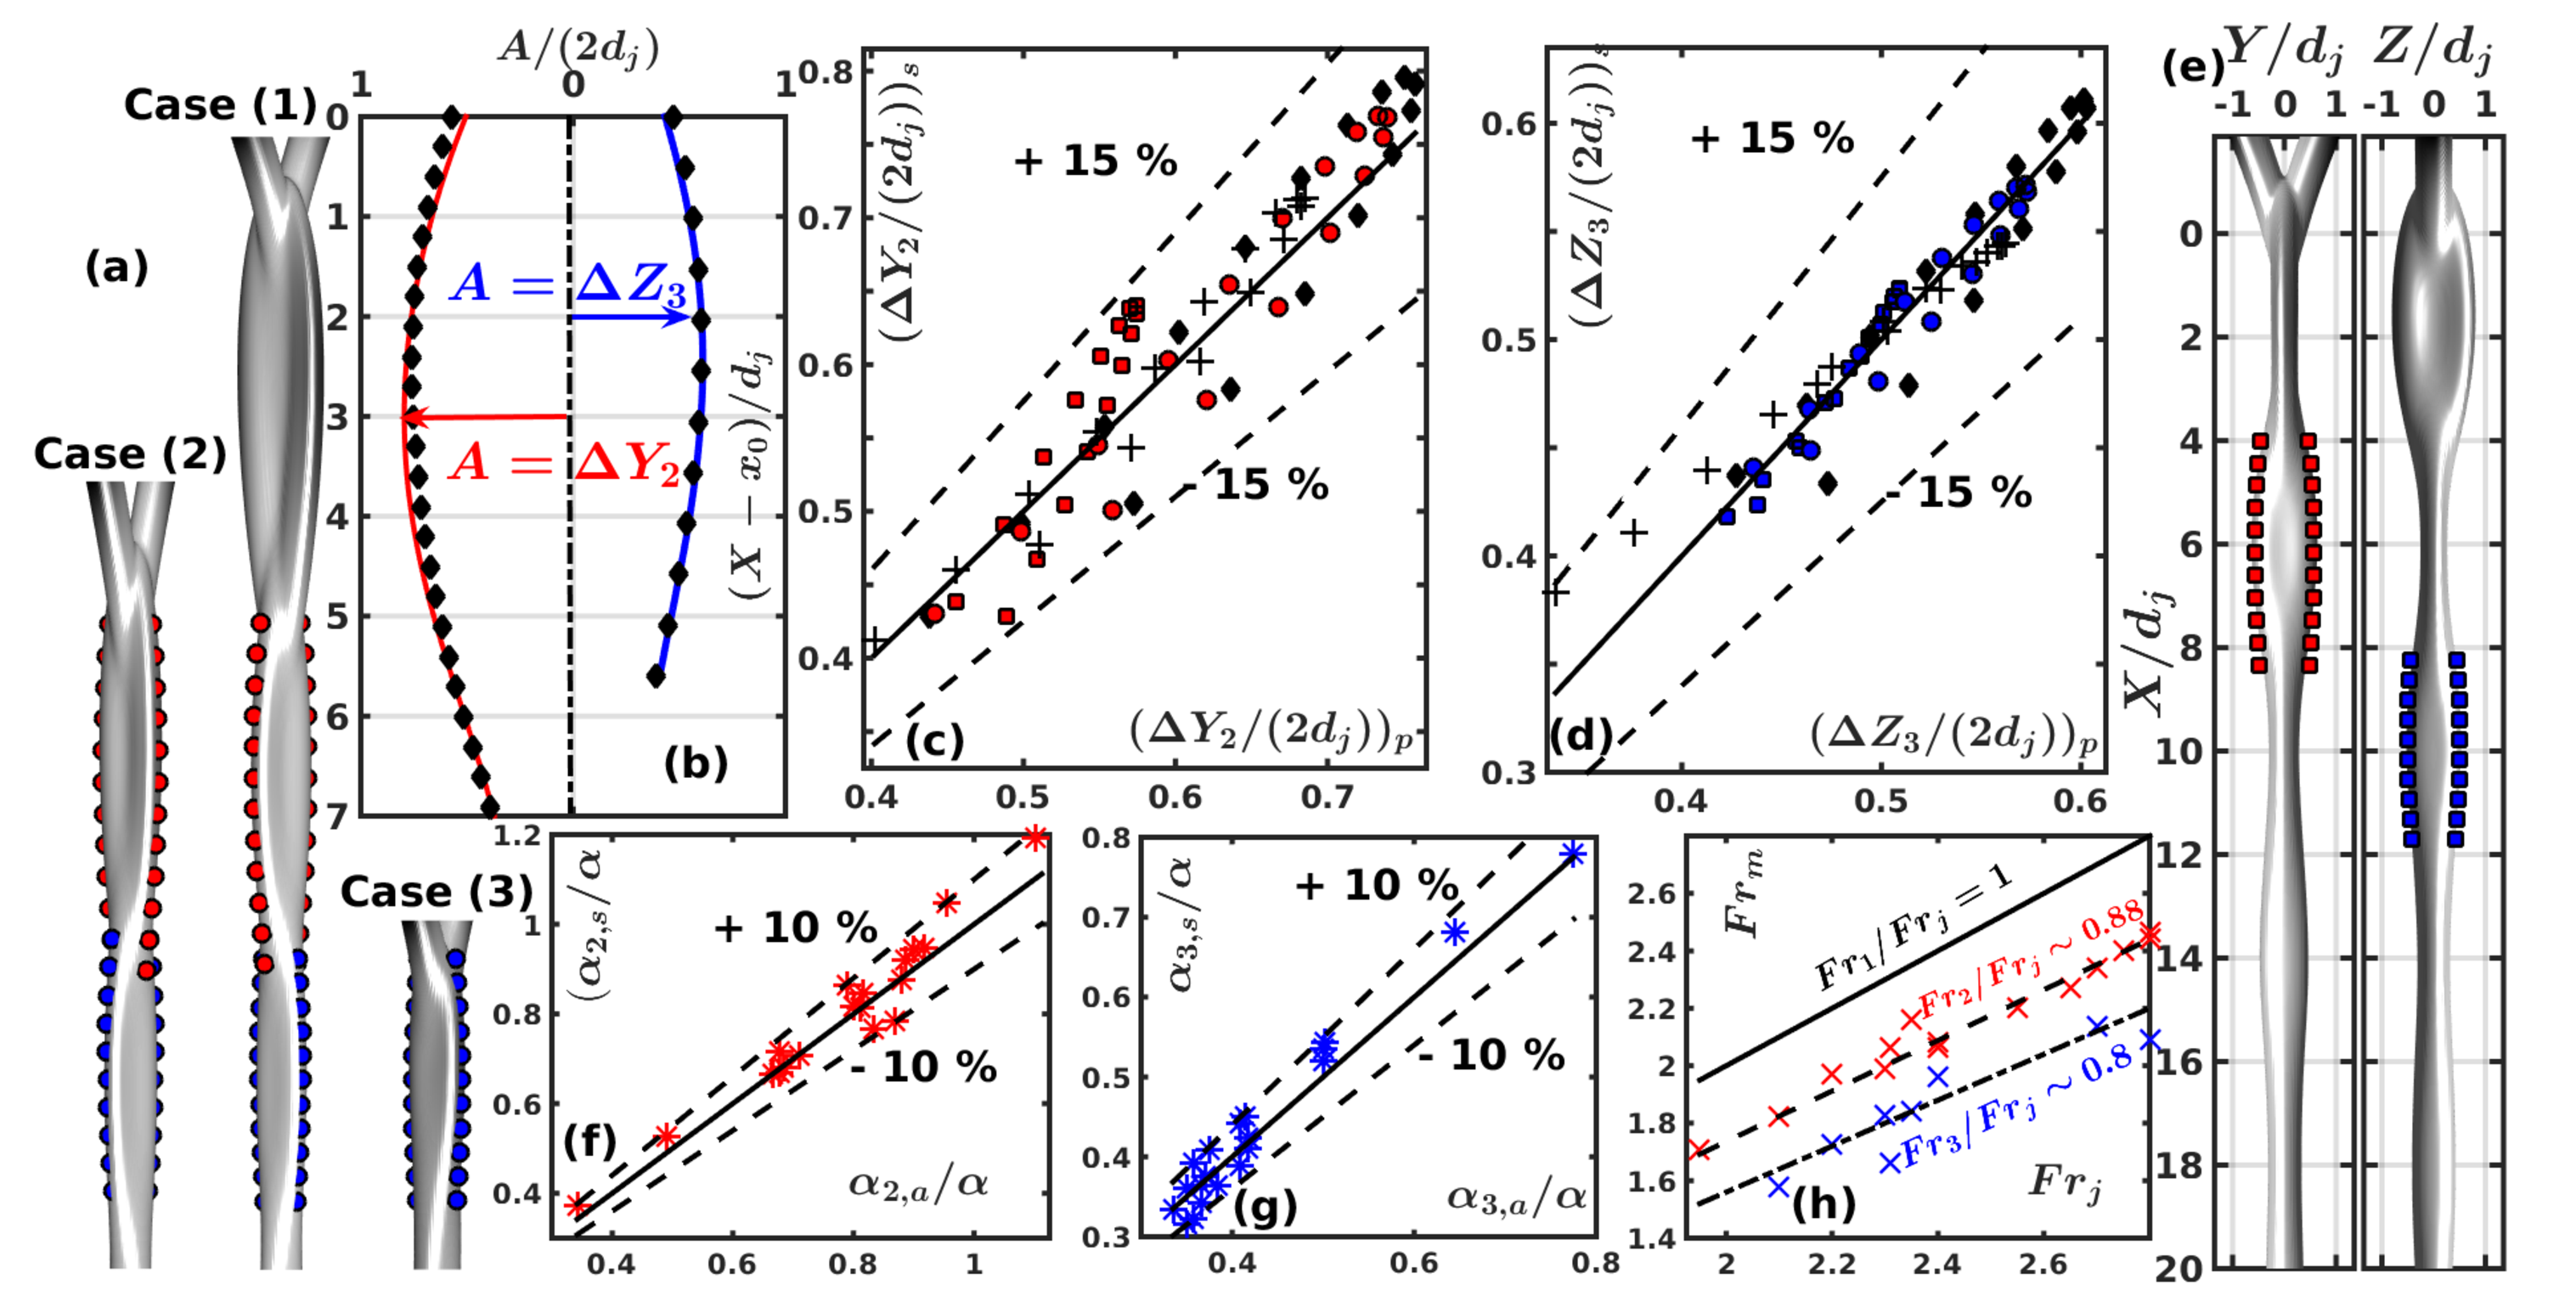
\includegraphics[width=\linewidth]{secondCollision}
	\caption{}
	\label{Figure::secondCollision}
\end{figure}
\lipsum
\subsection{Characteristic variation of secondary and tertiary links}
\lipsum[1]
\begin{figure}
	\centering
	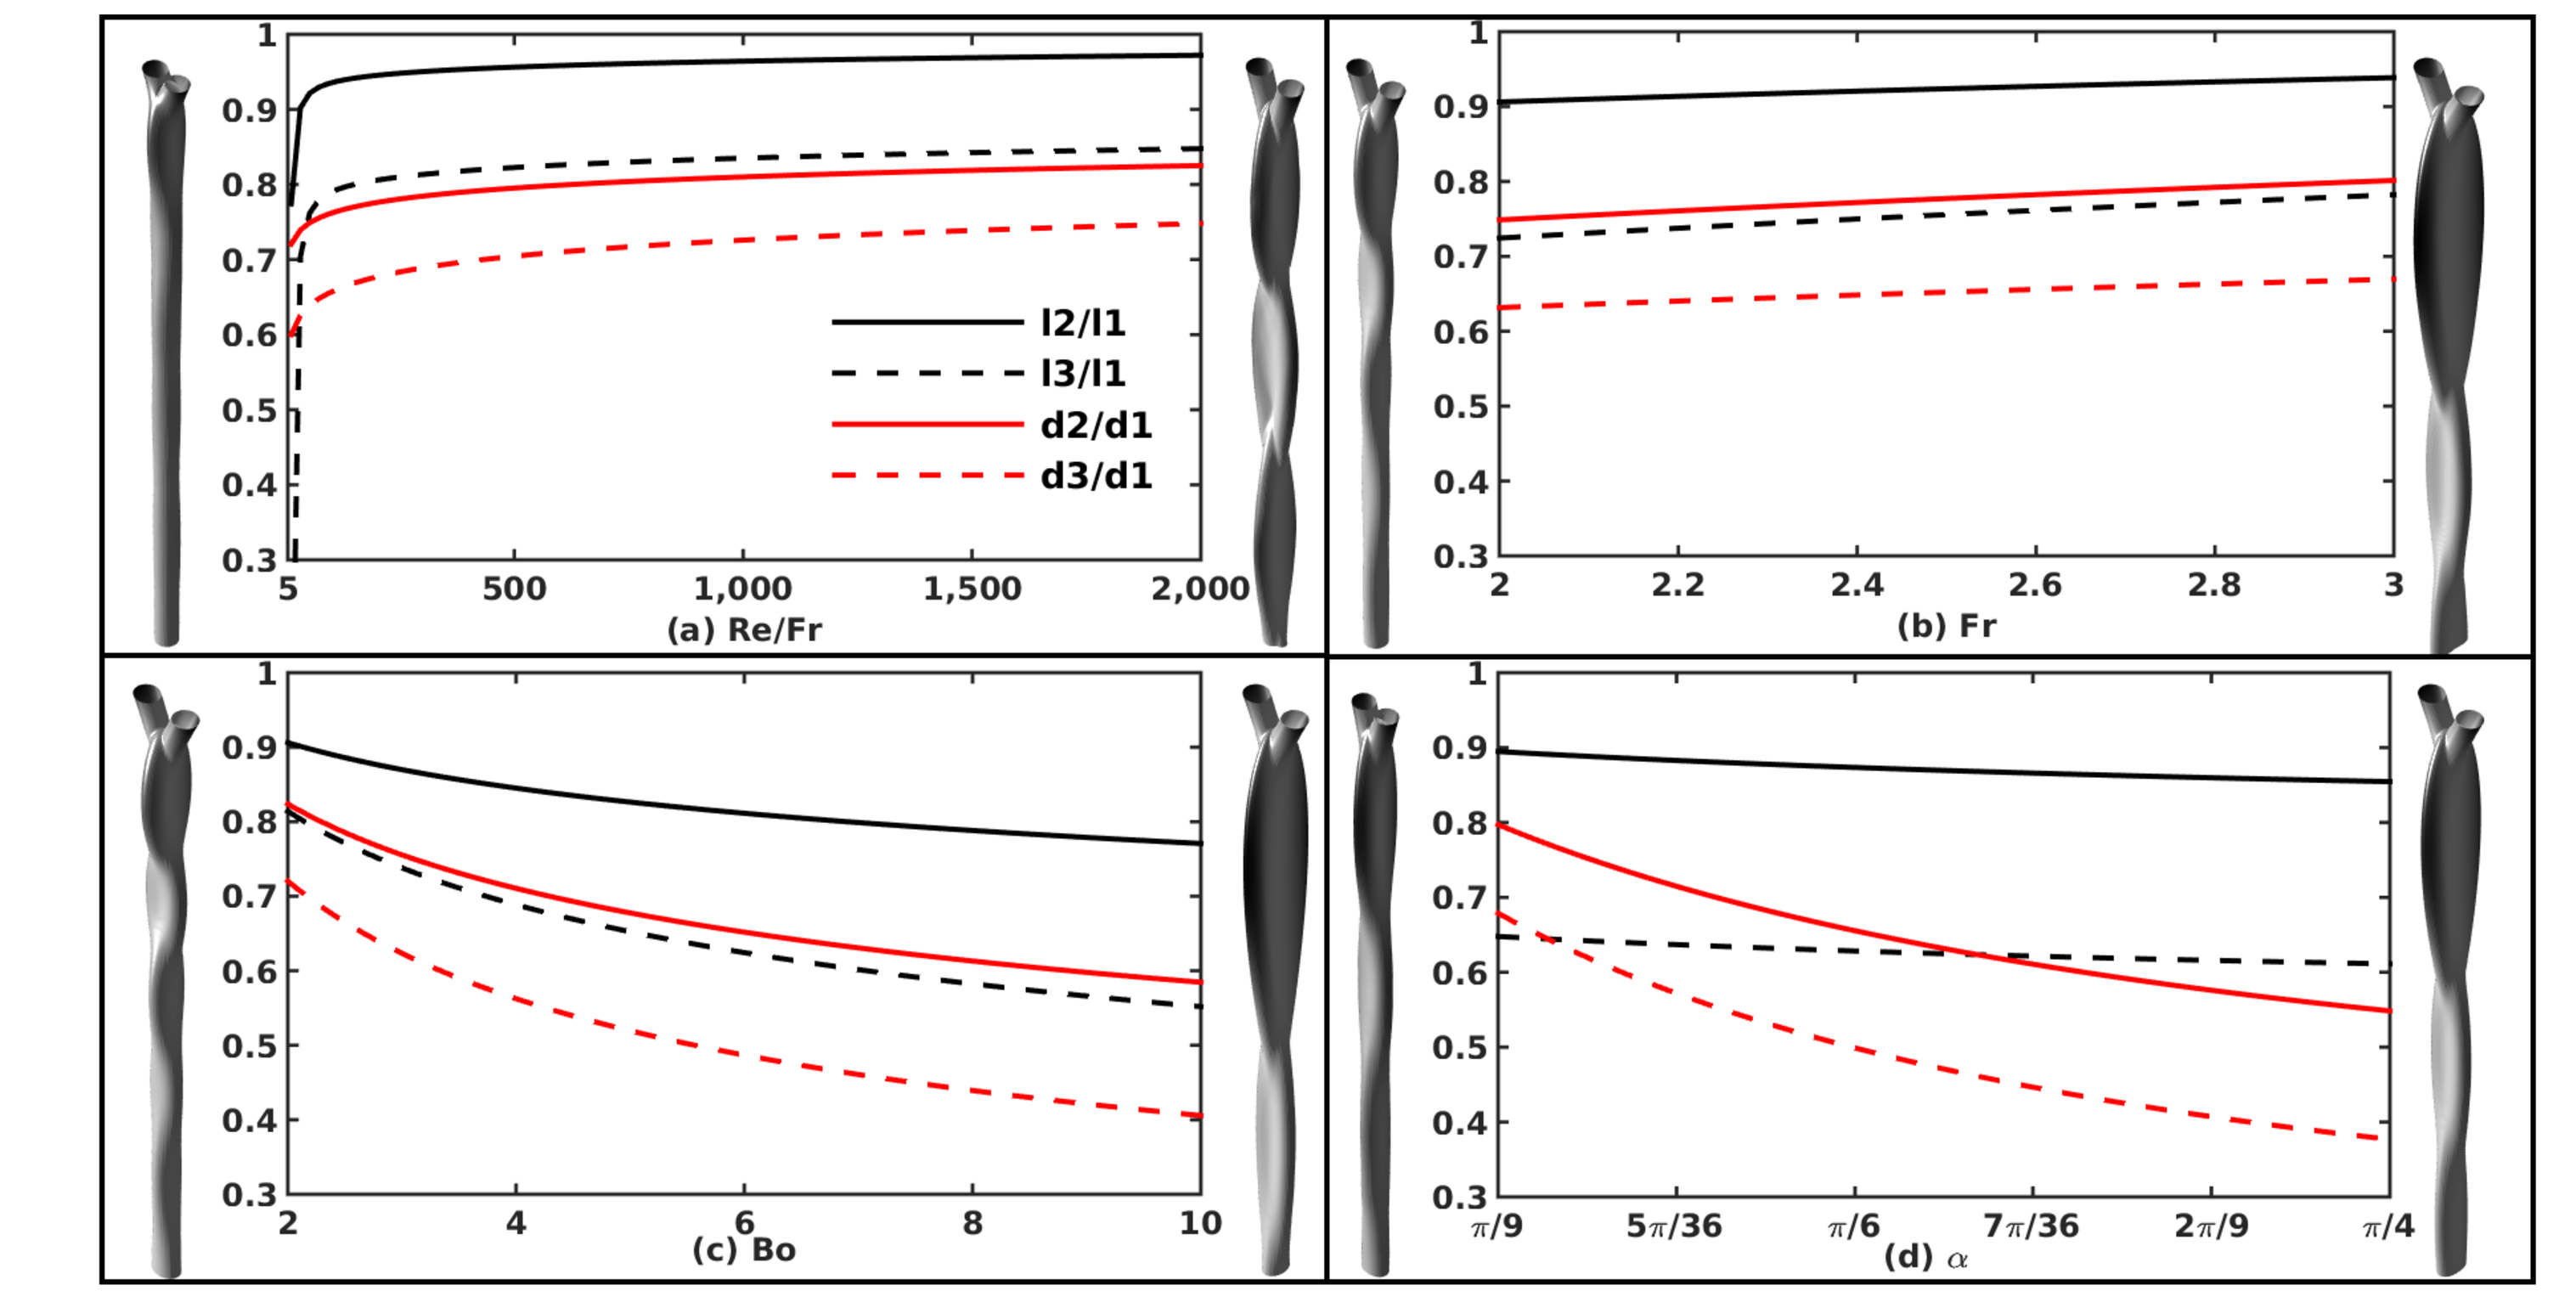
\includegraphics[width=\linewidth]{lil1did1}
	\caption{}
	\label{Figure::lil1}
\end{figure}
\lipsum
\section{Conclusions}
\lipsum[1]
\nocite{*}
\bibliography{chains}

\end{document}